\documentclass[a4paper,12pt]{book}

\usepackage{amssymb, amsmath, amsfonts, amsthm}
\usepackage{cite} % for citing from *.bib
\usepackage{color}
\usepackage{graphicx}
\usepackage{subfigure}
\usepackage{wrapfig}
\usepackage{xcolor}

\definecolor{shadecolor}{RGB}{200.,200.,200.}

\usepackage{pythonhighlight}
\usepackage{longtable}
\usepackage{todonotes}

\usepackage{tikz}

\usepackage{fourier} % snyggare font
\usepackage{appendix}

\usepackage{fixltx2e}

\usetikzlibrary{arrows,matrix,fit}
\usetikzlibrary{calc,3d}
\usetikzlibrary{shapes,snakes}

%% For theorems and the like: %%
\theoremstyle{plain}
\newtheorem{thm}[equation]{Theorem}
\newtheorem{Lemma}[equation]{Lemma}
\newtheorem{Proposition}[equation]{Proposition}
\newtheorem{Corollary}[equation]{Corollary}

\theoremstyle{definition}
\newtheorem{defi}[equation]{Definition}
\newtheorem{Remark}[equation]{Remark}
\newtheorem{Example}[equation]{Example}

%% Document %%
\begin{document}

\title{Grassmannians and Shape Space}
\author{Valentine Svensson}
\date{}

\maketitle

\tableofcontents

\chapter{Introduction} % (fold) 
\label{sec:introduction} 
In this work we will
investigate various ways of talking about multilinear algebra, what you get
when you consider several linear subspaces of a linear space, and relations
between them.

The central object at all of this is the Grassmannian, which we will introduce
later.

We will start by briefly describing the classical version of the Grassmmanians
as it is presented in \cite{MR0028055} by Hodge and Pedoe. After this we
consider the Grassmannian as described through the modern language of exterior
algebra, the primary reference for this section is \cite{MR1849803}. We shall
try to give the necessary information and theory for both sections. Now and
again we will mention some examples where the theory is used, and interesting
things that have come up while working with the theory.

We will later consider a coordinization of point configurations in space,
invariant under euclidean transformations, called \emph{Shape Spaces}. There
turns out to be a connection to the Grassmannian. A large part of this section
will also be devoted to trying to use the theory to get interesting results
about coordinzing grids in space.

There is also a section about Grassmann tensors, which is yet a generalization.
% section introduction (end)

\section{Previous work} % (fold)
\label{sec:previous_work}
The roots of this is from Julius Plucker who in \cite{plucker1828analytisch}
used a coordinatization for lines in projective 3-space to simplify analytical
line geometry. This was further developed in \cite{gh1844} where Hermann
Grassmann used a coordinatization for subspaces of a space. This
coordinatization lead to a point mapping of the manifold mentioned above.

The main inspiration for this thesis have been the shape space theory of Gunnar
Sparr et al and an interest in using multlinear algebra to do geometry.
Information about early work leading up to multilinear algebra is scattered
around the thesis in the form of ``history boxes''. Another facet of
multilinear algebra is a field called geometric algebra, marketed by Leo Dorst
et al as a way to do ``object oriented geometry'', mainly for use in
computation.  Multilinear algebra is more a tool than a source of questions and
problems in itself.

Regarding shape space, they where invented in the 90's as a way of
parametrizing the shapes of objects in images when doing scene reconstruction
from several known projection (images). Though there seem to be a publication
regarding shape spaces now and again, in later years they are not as popular as
other approaches to the problem.

% section previous_work (end)

\section{The Grassmannian} % (fold)
\label{sec:the_grassmannian}
The Grassmannian \( Gr(m,n) \) is the set of \( n \)-dimensional subspaces of
an \( m \)-dimensional vector space.
Alternatively, \( Gr(V,n) \) denotes the set of \( n \)-dimensional subspaces
of a particular vector
space \( V \) of dimension \( m \).
% section the_grassmannian (end)

\begin{figure}
	\tikzstyle{historybox} = [draw=black, fill=yellow!16, thick,
	rectangle, rounded corners, inner sep=10pt, inner ysep=20pt]
\begin{tikzpicture}
\node [historybox] (box){%
\begin{minipage}{\columnwidth}
	\textbf{August Ferdinand M\"obius (1790 - 1868)}
	As a researcher in Leipzig, M\"obius, who also worked a lot on Astronomy,
	published
	\emph{Der barycentrische Calcul} in 1827. A work on projective and affine
	geometry.
	In this work M\"obius introduced homogeneous coordinates and presented many
	results regarding
	projective transformations.
\end{minipage}
};
\end{tikzpicture}
\end{figure}

\begin{figure}
	\tikzstyle{historybox} = [draw=black, fill=yellow!16, thick,
	rectangle, rounded corners, inner sep=10pt, inner ysep=20pt]
\begin{tikzpicture}
\node [historybox] (box){%
\begin{minipage}{\columnwidth}
	\textbf{Hermann Grassmann (1809 - 1877)}
	To be allowed to teach mathematics and the natural sciences at higher level of school
	Grassmann needed to pass an examination process which included an essay on the physics
	of tides. While working on the essay Grassmann realized many parts of the known theory
	could be simplified using what we today would call vector analysis. This was in fact the
	first paper where even vector addition was defined and used.
	While a school teacher in Stettin, Grassmann developed the same insights to a new branch of
	mathematics	dubbed Linear Extension Theory (\emph{Lineale Ausdehnungslehre}), which he
	described in a book published 1844. Here Grassmann treated points lines and planes as
	algebraic objects, manipulatable by certain fundamental relations.
	Grassmann worked much as modern linear algebra texts, defining basis vectors allowed
	to span spaces, leading to the study of linear independence, and eventually subspace theory.
	He viewed linear spaces in the way that we today think of the Grassmann manifold.
	Based on Grassmanns work, Peono introduced vector spaces as we know them in 1888.
\end{minipage}
};
\end{tikzpicture}
\end{figure}

\begin{figure}
	\tikzstyle{historybox} = [draw=black, fill=yellow!16, thick,
	rectangle, rounded corners, inner sep=10pt, inner ysep=20pt]
\begin{tikzpicture}
\node [historybox] (box){%
\begin{minipage}{\columnwidth}
	\textbf{William Kingdon Clifford (1845 - 1879)}
	After studying Grassmanns work as well as William Rowan Hamiltons work on
	quaternions, Clifford unified the theories of exterior algebras (due to
	Grassmann) and quaternions in to a single framework via a new kind of
	associative product called the \emph{geometric product}.
\end{minipage}
};
\end{tikzpicture}
\end{figure}

\begin{figure}
	\tikzstyle{historybox} = [draw=black, fill=yellow!16, thick,
	rectangle, rounded corners, inner sep=10pt, inner ysep=20pt]
\begin{tikzpicture}
\node [historybox] (box){%
\begin{minipage}{\columnwidth}
	\textbf{Giuseppe Peano (1858 - 1932)}
	In 1888 Peano published the book \emph{Geometrical Calculus}\footnote{This
	book also contained an introductory
	chapter on mathematical logic. This was the first work by Peano on the subject, which
	he later would be most known for.}, where he had
	modernized the theories of Grassmann in an effort to make them more clear
	and available for more people. The theories remained obscure still however, but
	the book contains a very early example of a modern definition of a vector space.
\end{minipage}
};
\end{tikzpicture}
\end{figure}

\chapter{Preliminaries}
\section{Grassmann coordinates} % (fold)
\label{sec:grassmann_coordinates}

Let \( V \) be an \( m \)-dimensional vector space. Then an \( n
\)-dimensional subspace \( W \) of \( V \) is determined by its
Grassmann coordinates. Grassmann coordinates are calculated by taking
a matrix \( M \) of size \( m \times n \) whose span is \( W \), and
calculating the determinants of all \( n \times n \) sub matrices of
\( M \). Or to be formal; let \( \sigma_i \) be the \( i \)'th ordered
(increasing) sequence of \( n \) integers in the range \( 1,...,m \).
Then we say that \( M_{\sigma_i} \) is the matrix consisting of the
rows in \( M \) whos numbers are specified by \( \sigma_i \). The
Grassmann coordinates of \( W \) are then
\[
     \left( |M_{\sigma_1}|, \ldots, |M_{\sigma_{m \choose n}}| \right).
\]

\begin{figure}
\centering
\subfigure[An \( m \times n \) matrix spanning a subspace]{
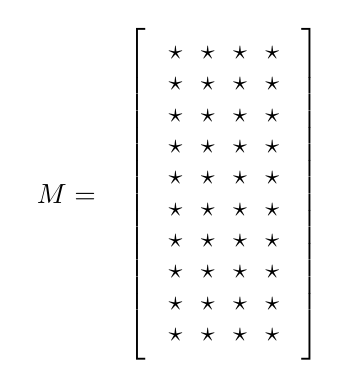
\begin{tikzpicture}

\node (G) {\( M = \)};

\matrix (M)
[matrix of math nodes,
 right of = G,
 xshift = 1cm,
 ampersand replacement = \&,
 left delimiter = \lbrack,
 right delimiter = \rbrack]
{
\star \& \star \& \star \& \star \\
\star \& \star \& \star \& \star \\
\star \& \star \& \star \& \star \\
\star \& \star \& \star \& \star \\
\star \& \star \& \star \& \star \\
\star \& \star \& \star \& \star \\
\star \& \star \& \star \& \star \\
\star \& \star \& \star \& \star \\
\star \& \star \& \star \& \star \\
\star \& \star \& \star \& \star \\
};

\end{tikzpicture}
}
\subfigure[An \( n \times n \) submatrix]{
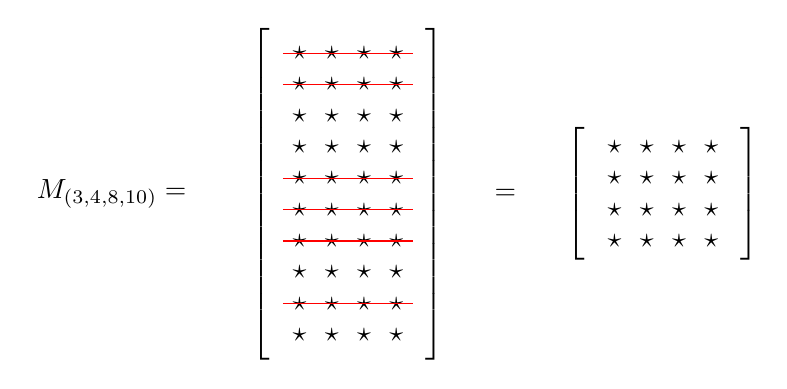
\begin{tikzpicture}

\node[xshift = -1cm] (G1) {\( M_{(3,4,8,10)} = \)};

\matrix (M)
[matrix of math nodes,
 right of = G1,
 xshift = 2cm,
 ampersand replacement = \&,
 left delimiter = \lbrack,
 right delimiter = \rbrack]
{
\star \& \star \& \star \& \star \\
\star \& \star \& \star \& \star \\
\star \& \star \& \star \& \star \\
\star \& \star \& \star \& \star \\
\star \& \star \& \star \& \star \\
\star \& \star \& \star \& \star \\
\star \& \star \& \star \& \star \\
\star \& \star \& \star \& \star \\
\star \& \star \& \star \& \star \\
\star \& \star \& \star \& \star \\
};

\draw[red] (M-1-1.west) to (M-1-4.east);
\draw[red] (M-2-1.west) to (M-2-4.east);
\draw[red] (M-5-1.west) to (M-5-4.east);
\draw[red] (M-6-1.west) to (M-6-4.east);
\draw[red] (M-7-1.west) to (M-7-4.east);
\draw[red] (M-9-1.west) to (M-9-4.east);

\node[right of = M, xshift = 1cm,] (G) {\( = \)};

\matrix (subM)
[matrix of math nodes,
 right of = G,
 xshift = 1cm,
 ampersand replacement = \&,
 left delimiter = \lbrack,
 right delimiter = \rbrack]
{
\star \& \star \& \star \& \star \\
\star \& \star \& \star \& \star \\
\star \& \star \& \star \& \star \\
\star \& \star \& \star \& \star \\
};

\end{tikzpicture}
}

\caption{Illustration of how to calculate Grassmann coordinates}

\end{figure}

% http://books.google.com/books?id=tVKzPSVAoEUC&printsec=frontcover
% &dq=editions:tVKzPSVAoEUC&hl=sv&ei=S-Z_TNy-
% KJOYOKqM6akO&sa=X&oi=book_result&ct=result&resnum=2&ved=0CC4Q6AEwAQ#v=onepage&q&f=false

\begin{thm}
	Each point in \( Gr(m,n) \) has a set of Grassmann coordinates which
	is unique up to a common multiplier.
\end{thm}
\begin{proof}
	\footnote{This proof is from \cite{MR0028055},
	starting at page 289. }
	Let \( V \in Gr(m,n) \). Say that \( V \) is determined by the basis
	\( A^i = ( \alpha_0^i, \ldots, \alpha_m^i) \) where
	\( i = 0, \ldots, n \). Assume that the Grassmann coordinates of
	\( V \) are
	\[
		( \ldots, p_{i_0 \cdots i_n}, \ldots).
	\]
	At least one of the coordinates is not zero; say
	\( p_{j_0 \cdots j_n} \not = 0 \). The condition for any point
	\( x_0, \ldots, x_m \) to lie in \( V \) is that the matrix
	\[
		\begin{bmatrix}
			\alpha_0^0 & \cdots & \alpha_m^0 \\
			\vdots & & \vdots \\
			\alpha_0^n & \cdots & \alpha_m^n \\
			x_0 & \cdots & x_m
		\end{bmatrix}
	\]
	should be of rank \( k+1 \).
	This means a matrix formed by taking the columns numbered
	\( i_0, \ldots, i_{k+1} \) will have determinant equal to zero.
	\[
		\begin{vmatrix}
			\alpha_{i_0}^0 & \cdots & \alpha_{i_{n+1}}^0 \\
			\vdots & & \vdots \\
			\alpha_{i_0}^n & \cdots & \alpha_{i_{n+1}}^n \\
			x_{i_0} & \cdots & x_{i_{n+1}}
		\end{vmatrix} = 0
	\]
	If we expand this determinant along the lowest row we get
	\[
		\sum_{h = 0}^{n + 1} (-1)^h x_{i_h}
		p_{i_0 \cdots i_{h-1} i_{h+1} \cdots i_{n+1}} = 0.
	\]
	These equations (for all possible choices of \( i_0, \ldots, i_{n+1} \))
	are either identically true, or define \emph{primes}\footnote{
		I think this means linear relations, the Google Books version
		of the book doesn't have an index to find definitions with.
	} which contain all points of \( V \).
	So all of these \( m+1 \choose n+1 \) equations defines a linear space
	which contains \( V \).
	We need to show that \( V \) is \emph{defined} by those equations.
	We show that among them is a set of \( m-n \) linearly
	independant equations.

	Consider the specific equation of this set where
	\[
		(i_0, \ldots, i_{n+1}) = (j_0, \ldots, j_n, j),
	\]
	and \( j \) is any integer in the range \( 0, \ldots, m \) but
	distinct from any \( j_0, \ldots, j_n \).
	That equation is
	\[
		\sum_{h = 0}^{n} (-1)^h x_{j_h}
		p_{j_0 \cdots j_{h-1} j_{h+1} \cdots j_{n} j}
		+ (-1)^{n+1} x_j p_{j_0 \cdots j_{n}} = 0 .
	\]
	Each Grassmann coordinate is skew-symmetric in its suffixes
	\footnote{This would be nice to have a proof of too.}.
	Thus the equation can be written
	\[
		\sum_{h = 0}^{n} (-1)^h x_{j_h} (-1)^{n-h}
		p_{j_0 \cdots j_{h-1} j j_{h+1} \cdots j_{n}}
		+ (-1)^{n+1} x_j p_{j_0 \cdots j_{n}} = 0 ,
	\]
	or
	\begin{equation}
	\label{eq:coeffs}
		x_j p_{j_0 \cdots j_{n}} -
		\sum_{h = 0}^{n} x_{j_h}
		p_{j_0 \cdots j_{h-1} j j_{h+1} \cdots j_{n}} = 0 .
	\end{equation}
	If \( (j_0, \ldots, j_n, j_{n+1}, \ldots, j_m) \) is a derangement
	of \( (0, \ldots, m) \) we consider the equations \ref{eq:coeffs}
	for the values of \( j \) given by \( j = j_{n+1}, \ldots, j_m \).
	The matrix of coefficients of these equations is an
	\( (m-n) \times (m+1) \) matrix \( M \).
	Now consider the the determinant of the submatrix of \( M \) created by
	taking the columns with suffixes \( j_{n+1}, \ldots, j_m \). It is equal to
	\( (p_{j_0 \cdots j_n})^{m-n} \), which is nonzero since we assumed that
	\( p_{j_0 \cdots j_n} \not = 0 \). This means the matrix \( M \) is of
	tank \( m-n \).
	So the set of equations (\ref{eq:coeffs}) defines \( m-n \) linearly
	independant primes. Therefore (\ref{eq:coeffs}) defines \( V \).
	This means the equations of \( V \) are determined by the Grassmann
	coordinates of \( V \), and it follows that no two distinct
	\( n \)-dimensional spaces can have the same coordinates.
\end{proof}

\begin{thm}[\cite{MR0028055}]
	Let \( \alpha_0, \ldots, \alpha_s \) be \( s+1 \) distinct integers so that
	\( s \leq k \) chosen between \( 0 \) and \( n \). Also let \( S_{n-s+1} \) be the linear
	space whose equations are
	\[
		x_{\alpha_0} = \cdots = x_{\alpha_s} = 0.
	\]
	Then \( S_k \) meets \( S_{n-s+1} \) in a space of dimension at least \( k-s \) if and only if
	\[
		p_{\alpha_0 \cdots \alpha_s i_{s+1} \cdots i_k} = 0
	\]
	for all possible choices of \( i_{s+1}, \ldots, i_k \).
\end{thm}

\begin{thm}[\cite{MR0028055}]
	Let \( p_{\alpha_0 \cdots \alpha_k} \) be a nonzero Grassmann coordinate. Define
	\begin{equation}
		\label{xij}
		x_j^i = p_{\alpha_0 \cdots \alpha_{i-1} j \alpha_{i+1} \cdots \alpha_k}
	\end{equation}
	where \( i = 1, \ldots, k \) and \( j = 0, \ldots, n \)., also define
	\[
		B^i = (x_0^i, \ldots, x_n^i).
	\]
	Then
	\begin{enumerate}
		\item The point \( B^i \) is the unique point of intersection between \( S_k \) and
		\( S_{n-k} \).
		\item The collection \( B^0, \ldots, B^k \) form a basis for \( S_k \).
	\end{enumerate}
\end{thm}

\begin{Corollary}[\cite{MR0028055}]
	There exist a non-zero number
	\footnote{Or element in the field the linear space is defined over. I have not decided what
	level of abstraction all of this should be written in.}
	\( \rho \) such that
	\[
		\rho \cdot p_{i_0 \cdots i_k} =
		\begin{vmatrix}
			x_{i_0}^0 & \cdots & x_{i_k}^0 \\
			\vdots & & \vdots \\
			x_{i_0}^k & \cdots & x_{i_k}^k
		\end{vmatrix}
	\]
	for all possible choices of \( (i_0, \ldots, i_k) \).
\end{Corollary}

\begin{defi}[\footnote{Explanation to be made at another time}]
	The set of \( {n+1} \choose {n-k} \)-tuples
	\[
		(\ldots, p^{i_1 \cdots i_{n-k}}, \ldots)
	\]
	are called the \emph{dual Grassmann coordinates} of a linear space \( S_k \).
\end{defi}

\begin{thm}[\cite{MR0028055}]
	Recall the definition of \( x_j^i \) from (\ref{xij}). Now also define
	\[
		u_j^i = p^{\alpha_{k+1} \cdots \alpha_{j-1} i \alpha_{j+1} \cdots a_n}.
	\]
	We have these relations between \( x_j^i \) and \( u_j^i \):
	\begin{enumerate}
		\item If \( j > k \) and \( i \leq k \), then
		\[
			u_j^{\alpha_j} = p^{\alpha_{k+1} \cdots \alpha_n} =
			p_{\alpha_0 \cdots \alpha_k} = x_{\alpha_i}^i .
		\]
		\item If \( i,j > k \) where \( i \neq j \), and \( l,m \leq k \) where \( l \neq m \), then
		\[
			u_j^{\alpha_i} = 0 = x_{\alpha_m}^i .
		\]
		\item If \( i > k \) and \( j \leq k \), then
		\[
			u_j^{\alpha_j} = p^{\alpha_{k+1} \cdots \alpha_{i-1} \alpha_j \alpha_{i+1}
			\cdots \alpha_n} = -p_{\alpha_0 \cdots \alpha_{j-1} \alpha_i \alpha_{j+1}
			\cdots \alpha_n} = -x_{\alpha_i}^j .
		\]
	\end{enumerate}
\end{thm}

\begin{thm}
	Let \( S_h \) have the coordinates \( (\ldots, p_{i_0 \cdots i_h}, \ldots) \)
	and \( S_k \) have the dual
	coordinates \( (\ldots, q^{i_{k+1} \cdots i_n}, \ldots ) \). The two subspaces \( S_h \) and
	\( S_k \) have a subspace of dimension at least \( t \) in common if and only if
	\[
		\sum_{\lambda_1, \ldots, \lambda_s}
		q^{\alpha_{k+1} \cdots \alpha_{n-s} \lambda_1 \cdots \lambda_s}
		p_{\lambda_1 \cdots \lambda_s \beta_0 \cdots \beta_{h-s} } = 0 ,
	\]
	for any choices of \( \alpha_{k+1}, \ldots, \alpha_{n-s} \) and \( \beta_0, \ldots, \beta_{h-s} \),
	where \( s = h - t + 1 \).
\end{thm}

\begin{thm}
	Again let \( S_h \) have the coordinates \( (\ldots, p_{i_0 \cdots i_h}, \ldots) \)
	and \( S_k \) have the coordinates \( (\ldots, q_{i_{0} \cdots i_k}, \ldots ) \).
	Assume they do not meet, then the Grassmann coordinates of the join of the two
	spaces \( S_h \) and \( S_k \) are \( ( \ldots, r_{i_0, \cdots, i_{h+k+1}}, \ldots ) \)
	where
	\[
		r_{i_0, \cdots, i_{h+k+1}} = \sum_j
		sign(j) \cdot p_{j_0 \cdots j_h} q_{j_{h+1} \cdots j_{h + k + 1}}.
	\]
	The sum is over all derangements \( j \) of \( (i_0, \ldots, i_{h+k+1}) \).
\end{thm}

\begin{defi}
	The \emph{quadratic \( p \)-relations} are
	\[
		p_{i_0 \cdots i_k} p_{j_0 \cdots j_k} =
		\sum_{\lambda = 0}^k p_{i_0 \cdots i_{s - 1} j_{\lambda} i_{s + 1} \cdots i_k}
		p_{j_0 \cdots j_{\lambda - 1} i_s j_{\lambda + 1} \cdots j_k} .
	\]
\end{defi}

\begin{thm}
	If all \( {n+1} \choose {k+1} \) elements of an ordered sequence
	\( (\ldots, p_{i_0 \cdots i_k}, \ldots) \) are skew-symmetric in the suffixes and satisfy
	the quadratic \( p \)-relations then the ordered sequence is the Grassmann coordinates of
	some subspace.
\end{thm}

\subsection{Regarding determinants} % (fold)
\label{sub:regarding_determinants}

Let the \emph{interior} of a matrix \( M \) be the submatrix of \( M \) where the first and last
rows and columns are removed. Another term commonly used for ``submatrix'' is \emph{minor}.
By \emph{consecutive minor} one means a minor whose rows and columns where all adjecant in the
original
matrix. For example, the interorior will be a consecutive minor.

\begin{thm}[Dodgsons Condensation Method]
	We can calculate the determinant of \( M \) by the following scheme:
	Form \( M^{(0)} \) by removing all zeros in the interior of \( M \) via elementary row or
	column operations.
	In the first step, form the \( (n-1) \times (n-1) \) matrix \( M^{(1)} \) by calculating all the
	\( 2 \times 2 \) consecutive minors of \( M^{(0)} \). In the following steps, say step \( k \),
	make \( M^{(k+1)} \) by calculating all \( 2 \times 2 \) minors of \( M^{(k)} \), and then
	 dividing
	all elements of \( M^{(k+1)} \) by the corresponding element in the interior of \( M^{k-1} \).
	Keep doing this until we are left with a single number, which will be the determinant.
\end{thm}

\begin{Example}
	Let us use the condesnation method to calculate the determinant of
	\[
		A = \begin{bmatrix}
			2 & 3 & 5 & 7 \\
			0 & 0 & -1 & -1 \\
			0 & -1 & -1 & 0 \\
			-2 & -3 & -4 & -7
		\end{bmatrix}.
	\]
	First, since there is a zero in the interior of \( A \) we perform the elementary row operation
	of switching the two top rows. Following that we get this iteration:
	\[
		A^{(0)} = \begin{bmatrix}
			0 & 0 & -1 & -1 \\
			2 & 3 & 5 & 7 \\
			0 & -1 & -1 & 0 \\
			-2 & -3 & -4 & -7
		\end{bmatrix}
	\]
	\[
		A^{(1)} = \begin{bmatrix}
			\begin{vmatrix}
				0 & 0 \\ 2 & 3
			\end{vmatrix} & \begin{vmatrix}
				0 & -1 \\ 3 & 5
			\end{vmatrix} & \begin{vmatrix}
				-1 & -1 \\ 5 & 7
			\end{vmatrix} \\ & & \\ \begin{vmatrix}
				2 & 3 \\ 0 & -1
			\end{vmatrix} & \begin{vmatrix}
				3 & 5 \\ -1 & -1
			\end{vmatrix} & \begin{vmatrix}
				5 & 7 \\ -1 & 0
			\end{vmatrix} \\ & & \\ \begin{vmatrix}
				0 & -1 \\ -2 & -3
			\end{vmatrix} & \begin{vmatrix}
				-1 & -1 \\ -3 & -4
			\end{vmatrix} & \begin{vmatrix}
				-1 & 0 \\ -4 & -7
			\end{vmatrix}
		\end{bmatrix} = \begin{bmatrix}
			0 & 3 & -2 \\ -2 & 2 & 7 \\ -2 & 1 & 7
		\end{bmatrix}
	\]
	\[
		A^{(2)} = \begin{bmatrix}
			\frac{\begin{vmatrix}
				0 & 3 \\ -2 & 2
			\end{vmatrix}}{3} & \frac{\begin{vmatrix}
				3 & -2 \\ 2 & 7
			\end{vmatrix}}{5} \\ & \\ \frac{\begin{vmatrix}
				-2 & 2 \\ -2 & 1
			\end{vmatrix}}{-1} & \frac{\begin{vmatrix}
				2 & 7 \\ 1 & 7
			\end{vmatrix}}{-1}
		\end{bmatrix} = \begin{bmatrix}
			2 & 5 \\ -2 & -7
		\end{bmatrix}
	\]
	\[
		A^{(3)} = \frac{\begin{vmatrix}
			2 & 5 \\ -2 & -7
		\end{vmatrix}}{2} = 2 = |A| .
	\]
\end{Example}
The usual way to (exactly) calculate the determinant of a matrix is by so
called \emph{Laplacian expansion}, but the condensation method have an edge in 
that
it generally requires fewer multiplications. Let us count! In the previous
example we performed
\[
	9 \cdot 2 + 4 \cdot 3 + 1 \cdot 3 = 33
\]
multiplications (if we count divisions as multiplications).
We compare this to Laplacian expansion of the same matrix (though we spare
ourselves having to spell it out), where we perform
\[
	4 + 4 \cdot (3 + 3 \cdot 2) = 40
\]
multiplications.

\begin{thm}[Cauchy-Binet]
	Let \( A \) be an \( m \times n \) matrix and \( B \) be an \( n \times m \) matrix.
	Then
	\[
		|AB| = \sum_\sigma |(A^T)_\sigma| |B_\sigma|
	\]
\end{thm}

% subsection regarding_determinants (end)

\begin{Corollary}
If a square matrix is divided in to two blocks, as
\( \begin{bmatrix}
	A & B
\end{bmatrix} \), then its determinant can be calculated by
\footnote{This is mentioned in \cite{rih_fs_2004}, but
no proof or reference is given. I will try to find a reference.}
\begin{equation}
	\label{eq:detformula}
	\begin{vmatrix}
		A & B
	\end{vmatrix} = \sum_\sigma \text{sign}(\sigma) \cdot
	|A_\sigma| \cdot |B_{-\sigma}|.	
\end{equation}
\end{Corollary}

% section grassmann_coordinates (end)

\chapter{Exterior algebra}

To combine vectors in a meaningful way, we define the wedge product for basis vectors.
To use it for anything else than basis vectors we let it be distributive, and we let
\[
	e_i \wedge e_i = 0,
\]
from which we can immediatly infer that
\[
	e_i \wedge e_j = - e_j \wedge e_i.
\]
The wedge product of two basis vectors will give a basis vector in the exterior power
\( \Lambda^2 V \)
of the vector space \( V \).
Wedging several basis vectors \( e_{i_1}, \ldots, e_{i_k} \) like
\[
	e_{i_1} \wedge \cdots \wedge e_{i_k}
\]
will give a basis vector in the
exterior product \( \Lambda^k V \).
The direct sum
\[
	\Lambda^0 V \oplus \Lambda^1 V \oplus \cdots \oplus \Lambda^{k-1} V \oplus \Lambda^k V = \Lambda V
\]
forms the exterior algebra \( \Lambda V \) of the vector space \( V \)

\section{Exterior Algebra formulation} % (fold)
\label{sec:exterior_algebra_formulation}
The reference for this section is \cite{MR1849803}.
\begin{defi}
	Let \( W \) be an \( m \)-dimensional linear subspace spanned by \( a_1, \ldots, a_m \).
	If we compute \( a = a_1 \wedge \cdots \wedge a_m =
	\sum_{i_1 < \cdots < i_m} \alpha_{i_1 \cdots i_m} e_{i_1} \wedge \cdots \wedge e_{i_m} \), then
	we define the coefficients \( \alpha_{i_1 \cdots i_m} \) to be the \emph{Grassmann coordinates}
	of \( W \).
\end{defi}

\begin{defi}
	If \( b = a_1 \wedge \cdots \wedge a_m \) where \( b \in \Lambda^m V \) for some
	\( a_1, \ldots, a_m \in V \) we say that \( b \) is \emph{simple}.
\end{defi}

\begin{thm}
	The set of simple elements of \( \Lambda^m V \) is an algebraic variety.
	Also, the set of one dimensional subspaces spanned by simple elements form a projective
	variety in the projective space over \( \Lambda^m V \).
\end{thm}
We call that projective variety the \emph{Grassmann variety} \( G_{n,k} \).
\begin{thm}
	A set of vectors \( \{a_1, \ldots, a_n\} \) are linearly dependant if and only if their exterior
	product \( a_1 \wedge \cdots \wedge a_n = 0 \).
\end{thm}
\begin{thm}[Pl{\"u}cker relations]
	Let \( V \) be a linear space of dimension \( n \) with basis \( e_1, \ldots, e_n \).
	Assume that elements \( a \in \Lambda^k V \) are written in the form
	\( a = \sum_{i_1 < \cdots < i_k} \alpha_{i_1 \cdots i_k} e_{i_1} \wedge \cdots \wedge e_{i_k} \)
	.
	If \( a \) is simple, then
	\[
		\sum_{s=0}^k (-1)^s a_{i_0 \cdots \not i_s \cdots i_k} a_{j_1 \cdots i_s \cdots j_{k-1}}
		= 0
	\]
	for all possible indices \( i_0 < \cdots < i_k \) and \( j_0 < \cdots < j_k \).
	The Grassmann coordinates which are undefined are set to zero.
	This set of equations defines the Grassmann variety.
\end{thm}
A little explenation on the notation here; we write \( \not i_s \) when we mean that \( i_s \)
is removed from the list. In the list in the second term the \( i_s \) is inserted at the
appropriate place.

\subsection{Brief stop at \( Gr(4,2) \)} % (fold)
\label{sub:brief_stop_at_inl}

Let us look at the example of linear spaces spanned by two
points in projective space \( \mathbb{PR}^3 \).
Such a space will represent a line in \( \mathbb{R}^3 \).
The space will have \( {4 \choose 2} \) coordinates,
and we denote these as \( (a_{01},a_{02},a_{03},a_{12},a_{13},a_{23}) \).
Let us start off this example by putting \( (i_0, i_1, i_2) = (0, 1, 2) \) and \( j_1 = 3 \).
Then the quadratic
relation corresponding to these indices will be
\begin{equation} \label{line_rel}
	a_{12}a_{03} - a_{02}a_{13} + a_{01}a_{23} = 0.
\end{equation}
Any polynomials where \( j_1 \in \{i_0, i_1, i_2\} \) will reduce to \( 0 \),
and it turns out that all
other polynomials will be equivalent to the one in equation \ref{line_rel}.
So the Grassmannian \( Gr (4,2) \) will be determined by equation \ref{line_rel}.
Let us make this even more concrete by calculating the Grassmann
coordinates for a line and test the relation.
The points spanning the line will be
\[
	\begin{bmatrix}
		4 \\ 1 \\ 1 \\ 1
	\end{bmatrix} \text{ and } \begin{bmatrix}
		1 \\ 2 \\ 3 \\1
	\end{bmatrix},
\]
so we calculate the Grassmann coordinates to the span of the matrix
\[
	\begin{bmatrix}
		4 & 1 \\ 1 & 2 \\ 1 & 3 \\ 1 & 1
	\end{bmatrix},
\]
and find them to be \( (7, 11, 3, 1, -1, -2) \). Now we can verify that
\[
	1 \cdot 3 - 11 \cdot (-1) + 7 \cdot (-2) = 0.
\]
This way of representing lines is usually called the \emph{Klein model} for lines,
and the coordinate representation, that is, Grassmann coordinates for this specific
Grassmannian, is called \emph{Pl\"ucker coordinates}. Let us concentrate on this
Grassmannian for a while. It is interesting in the sense that it is the Grassmannian
of smallest dimension which is not simply a projective space.
\begin{figure}
\tikzstyle{historybox} = [draw=black, fill=yellow!16, thick,
	rectangle, rounded corners, inner sep=10pt, inner ysep=20pt]
\begin{tikzpicture}
\node [historybox] (box){%
\begin{minipage}{\columnwidth}
	\textbf{Julius Pl\"ucker (1801 - 1868)}

	Pl\"ucker was a german geometer and physicist. Most of his work regarded analytical
	geometry of conic sections. In his work \emph{Analytisch-geometrische Entwickelungen},
	he used a homogeneous coordinate system for lines like we in this work call
	\emph{Pl\"ucker coordinates}. By viewing conic sections as envelopes of lines he could use
	his line coordinates also for studying these.
\end{minipage}
};
\end{tikzpicture}
\end{figure}

Calculating the six two-by-two determinants which give the Pl\"ucker coordinates of
line spanned by two points is not particularly problematic. But for the sake of
completion, let us list the expression of the coordinates of a line spanned by two
arbitrary points
\[
	p = \begin{bmatrix}
		p_0 \\ p_1 \\ p_2 \\ p_3
	\end{bmatrix}, q = \begin{bmatrix}
		q_0 \\ q_1 \\ q_2 \\ q_3
	\end{bmatrix}.
\]
These are
\begin{alignat}{2}
	a_{01} = p_0 q_1 - p_1 q_0, \quad a_{02} = p_0 q_2 - p_2 q_0, \quad
	 a_{03} = p_0 q_3 - p_3 q_0, \label{lineplucker} \\
	a_{12} = p_1 q_2 - p_2 q_1, \quad a_{13} = p_1 q_3 - p_3 q_1, \quad
	 a_{23} = p_2 q_3 - p_3 q_2.
\end{alignat}

By using the exterior algebra representation of of these coordinates we can solve some
practical problems using these coordinates.
\begin{Example}
	\textbf{Finding whether a point lies on a line.}
	The basis of the lines is
	\[ \{ e_0 \wedge e_1, e_0 \wedge e_2, e_0 \wedge e_3,
	e_1 \wedge e_2, e_1 \wedge e_3, e_2 \wedge e_3 \}. \] Say that the line in question
	is spanned by the points \( a \) and \( b \) via \( a \wedge b \), we want to see
	whether the point \( c \) lies on the line. Or in other words, if \( \{a,b,c\} \)
	are linearly dependant. Thus what we need to check is if
	\[
		a \wedge b \wedge c = 0.
	\]
	Since we will end up in the space \( \Lambda^3 \mathbb{R} \) after we have done
	those three products, we need to see that the coefficients become zero for all
	the basis vectors
	\[ \{ e_0 \wedge e_1 \wedge e_2, e_0 \wedge e_1 \wedge e_3,
	e_0 \wedge e_2 \wedge e_3, e_1 \wedge e_2 \wedge e_3 \}. \]
	Associativity and anti-commutativity of wedge products give us the relations
	\begin{align*}
		e_0 \wedge e_1 \wedge e_2 &= e_1 \wedge e_2 \wedge e_0 = - e_0 \wedge e_2 \wedge e_1, \\
		e_0 \wedge e_1 \wedge e_3 &= e_1 \wedge e_3 \wedge e_0 = - e_0 \wedge e_3 \wedge e_1, \\
		e_0 \wedge e_2 \wedge e_3 &= e_2 \wedge e_3 \wedge e_0 = - e_0 \wedge e_3 \wedge e_2, \\
		e_1 \wedge e_2 \wedge e_3 &= e_2 \wedge e_3 \wedge e_1 = - e_1 \wedge e_3 \wedge e_2.
	\end{align*}
	So imagine the line has coordinates \( (l_{01}, l_{02}, l_{03}, l_{12}, l_{13}, l_{23}) \),
	and the point we wish to check if it lies on the line has coordinates
	\( (c_0, c_1, c_2, c_3) \). Then by wedging the different coordinates and applying the relations
	stated above, we arrive at the system
	\begin{align*}
		l_{12} c_0 - l_{02} c_1 + l_{01} c_2 &= 0 \\
		l_{13} c_0 - l_{03} c_1 + l_{01} c_3 &= 0 \\
		l_{23} c_0 - l_{03} c_2 + l_{02} c_3 &= 0 \\
		l_{23} c_1 - l_{13} c_2 + l_{12} c_3 &= 0,
	\end{align*}
	which need to be satisfied for \( c \) to lie on the line \( L \).
	\begin{Example}
		For a concrete example, let us perform this for the points
		\[
			a = \begin{bmatrix}
				1 \\ 2 \\ 4 \\ 1
			\end{bmatrix}, b = \begin{bmatrix}
				1 \\ 5 \\ 3 \\ 1
			\end{bmatrix}, c = \begin{bmatrix}
				1 \\ 8 \\ 2 \\ 1
			\end{bmatrix}.
		\]
		We calculate the line \( L = a \wedge b = (3, -1, 0, -14, -3, 1) \) and plug this and
		\( c \) in to the system above to see whether \( c \in L \). The system becomes
		\begin{align*}
			-14 + 8 + 6 &= 0 \\
			-3 - 0 + 3 &= 0 \\
			1 - 0 - 1 &= 0 \\
			8 + 6 - 14 &= 0,
		\end{align*}
		which is satisfied.
	\end{Example}
\end{Example}
\subsection{An example: The set of lines in space is equivalent to the product
of two circles.} % (fold)
\label{sub:connection_to_quaternion_algebra}
Let us consider the exterior power \( \Lambda^4 \mathbb{PR}^3 \), this will only
consist of one basis vector; \( e_0 \wedge e_1 \wedge e_2 \wedge e_3 \), which
will be the orientation of \( \mathbb{PR}^3 \). Here we are looking at planes
in \( \mathbb{PR}^3 \), and now let us specifically look at oriented planes.
Now the Pl\"ucker coordinates of an oriented plane will in addition to the
quadratic Pl\"ucker relations
\begin{equation} \label{line_rel}
	a_{12}a_{03} - a_{02}a_{13} + a_{01}a_{23} = 0
\end{equation}
also satisfy
\[
	\sum a_{ij}^2 = 1.
\]
By simply performing the linear change of variables
\begin{alignat*}{2}
	x_1 = a_{12} + a_{34} \quad & x_2 = a_{14} + a_{23} \quad & x_3 = -a_{13} + a_{24} \\
	y_1 = a_{12} - a_{34} \quad & y_2 = -a_{14} + a_{23} \quad & y_3 = -a_{13} - a_{24}
\end{alignat*}	
we will get a set of coordinates which satisfies the relations
\[
	\sum x_i^2 = \sum y_i^2 = 1.
\]
This means that the coordinates of a line written with coordinates
\( (x_1, x_2, x_3, y_1, y_2, y_3) \) will lie in the product space
\( S^2 \times S^2 \), which is a four dimensional subspace of
\( \mathbb{R}^6 \).
Let \( P \in \Lambda^2 \mathbb{PR}^3 \) with orthonormal basis \( \{f_1, f_2\} \).
We view \( f_1 \) and \( f_2 \) as quaternions, so that
\begin{align*}
	f_1 = b_1 + b_2 i + b_3 j + b_4 k, \\
	f_2 = c_1 + c_2 i + c_3 j + c_4 k.
\end{align*}
In the three dimennsional subspace of quaternions with zero real part, a quaternion
lies on the unit sphere \( S^2 \) precisely when it is unit length.
As we assumed orthonormality, we have \( <f_1, f_2> = 0 \). Because of this
it follows that \( <f_1 \overline{f_1}, f_2 \overline{f_1}> = 0\).
So \( f_2 \overline{f_1} \) will lie on the unit sphere, the same argument holds for
\( \overline{f_2} f_1 \).

Consider now the mappings \( F \) and \( F' \) defined by \( F(x, y, z) = (x, -z, y) \)
and \( F'(x, y, z) = (-x, z, y) \).
Looking closer, we see that
\begin{align*}
	f_2 \overline{f_1} &= (c_1 + c_2 i + c_3 j + c_4 k)(b_1 - b_2 i - b_3 j - b_4 k) \\
	&= c_1 b_1 - c_1 b_2 i - c_1 b_3 j -
	c_1 b_4 k + b_2 a_1 i + c_2 b_2 - c_2 b_3 k + c_2 b_4 j \\
	& \quad + c_3 b_1 j + c_3 b_2 k + c_3 b_3 - c_3 b_4 i + c_4 b_1 k - c_4 b_3 i + c_4 b_4 \\
	&= (b_1 c_1 + b_2 c_2 + b_3 c_3 + b_4 c_4) + (b_1 c_2 - b_2 c_1 + b_3 c_4 - b_4 c_3) i \\
	& \quad + (b_1 c_3 - b_3 c_1 - b_2 c_4 + b_4 c_2) j
	+ (b_1 c_4 - b_4 c_1 + b_2 c_3 - b_3 c_2) k.
\end{align*}
By considering the quaternions as points in \( \mathbb{R}^4 \), and recalling the expressions
for the Pl\"ucker coordinates in equations \eqref{lineplucker}, we see that
\begin{align*}
	f_2 \overline{f_1} &= (b_1 c_1 + b_2 c_2 + b_3 c_3 + b_4 c_4) +
	(b_1 c_2 - b_2 c_1 + b_3 c_4 - b_4 c_3) i \\
	& \quad + (b_1 c_3 - b_3 c_1 - b_2 c_4 + b_4 c_2) j
	+ (b_1 c_4 - b_4 c_1 + b_2 c_3 - b_3 c_2) k \\
	&= (a_{12} + a_{34}) i + (a_{13} - a_{24}) j + (a_{14} + a_{23}) k \\
	&= x_1 i - x_3 j + x_2 k,
\end{align*}
where in the last equality we go back to the changed variables. We can do a similar
calculation going from \( \overline{f_2} f_1 \) to \(-y_1 i + y_3 j + y_2 k \).
Thus lines in space can be represented as points on \( S^2 \times S^2 \).


% subsection connection_to_quaternion_algebra (end)


\begin{defi}
	The \emph{annulator} of a linear subspace \( W \subset V \) is the set of all linear forms
	that vanish on \( W \). The annulator is a subspace of the dual space \( V^* \).
\end{defi}

\begin{defi}
	The \emph{dual Grassmann coordinates} of a linear (or projective) subspace are the Grassmann
	coordinates of its annullator space.
\end{defi}

\begin{defi}
	The linear operator \( * : \Lambda^k V \mapsto \Lambda^{n-k} V \) is defined as now described.
	Let \( e_{\wedge i_1 \cdots i_k} \) be a basis element for \( \Lambda^k V \), take
	\( j_1, \ldots, j_{n-k} \) as the complement of \( i_1, \ldots, i_k \). Thus
	\( (i_1, \ldots, i_k, j_1, \ldots, j_{n-k}) \) is a permutation of \( (1, \ldots, n) \).
	We define \( * \) by
	\[
		* e_{\wedge i_1 \cdots i_k} = \text{sign}(i_1, \ldots, i_k, j_1, \ldots, j_{n-k}) \cdot
		e_{\wedge j_1 \cdots j_{n-k}}.
	\]
\end{defi}

\begin{thm}
	Identify \( V \) and \( V^* \) by the bases \( e_1, \ldots, e_n \) and
	\( e_1^*, \ldots, e_n^* \) respectively. If \( a \in \Lambda^k V \) represents a linear
	(or projective) subspace, then \( * a \in \Lambda^{n-k} V \) represents its annullator space.
\end{thm}

\begin{thm}
	\label{findingspan}
	Let \( U \) be a linear subspace of \( V \) given by the basis
	\( \{a_1, \ldots, a_r\} \), and let
	\( W \)	be a linear subspace of \( V \) given by the basis \( \{b_1, \ldots, b_s\} \).
	The span
	\( U + W \) of the two subspacesis given by the basis
	\( \{a_1, \ldots, a_r, b_1, \ldots, b_s\} \).
	Let \( u = a_1 \wedge \cdots \wedge a_r \), and succesively compute
	\begin{itemize}
		\item \( u \wedge b_{i_1} \)
		\item \( u \wedge b_{i_1} \wedge b_{1_2} \)
		\item \( \cdots \)
	\end{itemize}
	and remove the sequences that result in zero until we have found a maximal sequence
	\( x = u \wedge b_{i_1} \wedge \cdots \wedge b_{i_k} \) such that \( x \wedge b_j = 0 \) for all
	\( j \).
	Then \( U + W \) is described by \( x \in \Lambda^{r+k} V \).
\end{thm}

\begin{thm}
	\label{dualrelation}
	Let \( U \) and \( W \) be linear subspaces of \( V \), and let \( T \) be their intersection
	\( T = U \cap W \). Then their duals satisfy \( T^* = U^* + V^* \).
\end{thm}

% section exterior_algebra_formulation (end)

\chapter{Shape space} % (fold)
\label{sec:shape_space}
\begin{defi}[\cite{sparr1998}]
	An \emph{\( n \)-point configuration} \( \mathcal{X}  \) is an ordered set of points
	\( \mathcal{X} = (X^1, \ldots, X^n) \) where every \( X^k \in \mathbb{A}^d \).
	Say that the \emph{dimension} \( \rho_\mathcal{X} \) of \( \mathcal{X} \) is the dimension of
	the smallest affine subspace which contains \( \mathcal{X}  \).
	Denote by \( \mathcal{C}_{n,\rho} \) the set of \( n \)-point configurations of dimension
	\( \rho \).
\end{defi}
The main motivation for shape spaces is to study relations between points with the coordinatization
abstracted away. For this, we make the following definition.
\begin{defi}
	Let \( X_a \) be an augmented coordinate matrix for \( \mathcal{X} \), then the \emph{affine
	shape space} \( s(\mathcal{X}) \) of \( \mathcal{X} \) is defined as
	\[
		s(\mathcal{X}) = \mathcal{N}(X_a),
	\]
	and the \emph{affine depth space} \( d(\mathcal{X}) \) is defined by
	\[
		d(\mathcal{X}) = \mathcal{R}_\text{row}(X_a).
	\]
\end{defi}
\begin{Lemma}[Fundamental lemma of shape spaces. ref: sparr1991]
	Let \( X_a \) and \( \overline{X_a} \) be augmented coordinate matrices of shape spaces
	related by an affine transformation \( T \) such that \( \overline{X_a} = T X_a \).
	Then \( \mathcal{N}(X_a) = \mathcal{N}(\overline{X_a}) \).
\end{Lemma}
\begin{proof}
	First, let us write \[
		T = \begin{bmatrix}
			A & b \\ 0 & 1
		\end{bmatrix}.
	\]
	Let the vector \( \xi = (\xi_1, \ldots, \xi_m) \) belong to \( \mathcal{N}(X_a) \), so that
	\( \sum_{i=0}^m \xi_i x^i = 0 \). Then
	\begin{align*}
		\sum_{i=0}^m \xi_i \overline{x^i} & = \sum_{i=0}^m \xi_i (A x^i + b) \\
		& = A \sum_{i = 0}^m \xi_i x^i + b \sum_{i = 0}^m \xi_i \\
		& = A \cdot 0 + b \cdot 0 = 0.
	\end{align*}
	So \( \xi \) must then also belong to \( \mathcal{N}(\overline{X_a}) \).
\end{proof}
Together with the following motivating theorem we will have a way of studying shapes affinely.
\begin{thm}[\cite{sparr1998}]
	Let \( \mathcal{X}, \overline{\mathcal{X}} \in \mathcal{C}_{n, \rho}\),
	then the following three
	statements are equivalent.
	\begin{itemize}
		\item The point configurations \( \mathcal{X} \) and \( \overline{\mathcal{X}} \) can be
		mapped onto each other by an affine transformation.
		\item \( s(\mathcal{X}) = s(\mathcal{\overline{X}}) \)
		\item \(  d(\mathcal{Y}) =  d(\mathcal{\overline{Y}}) \)
	\end{itemize}
\end{thm}
\begin{thm}
	Let X be a point configuration of \( m + 1 \) points with dimension
	dim X \( = \rho \). Then \( s(X) \in Gr(m - \rho, m) \)
\end{thm}
\begin{proof}
	\[
		dim X = \rho \rightarrow rank X_a = \rho + 1 \rightarrow
		dim N(X_a) = (m + 1) - (\rho + 1) = m - \rho.
	\]
\end{proof}
By \( \Sigma_0 \) we denote the vector space
\[
	\Sigma_0 = \left\{ ( x_1, \ldots, x_n ) \in \mathbb{R}^n \middle| \sum_{k=1}^n x_k = 0 \right\}
	\subset \mathbb{R}^n .
\]
We have the one to one correspondence
\[
	\mathcal{C}_{n,\rho} / \left\{\text{affine transformations} \right\}
	\cong Gr(\Sigma_0, n - \rho - 1).
\]

There is an isomorphism
\[
	Gr(\Sigma_0, n - \rho - 1) \cong Gr(\Sigma_0^\star, \rho + 1)
\]
which takes a linear subspace of dimension \( n - \rho - 1 \) 
to its orthogonal complement of
dimension \( \rho + 1 \).
Thus this isomorphism relates shape space to the corresponding depth space.

How to get the Grassmann coordinates of a depth space \( d( \mathcal{X} ) \):
Consider us having coordinate vectors for 
\( n \) points \(  X^1, \ldots, X^n \). The definition
of depth space is the row space of the augmented coordinate matrix
\[
	X_a = \begin{bmatrix}
		X^1 & \cdots & X^n \\
		1 & \cdots & 1
	\end{bmatrix}.
\]
That is, the span of the transposed augmented coordinate matrix \( X_a^T \). 
Thus we can compute
the Grassmann coordinates of the spanned space by the methods described above.

One part of the shape and depth theorem says that if 
\( \mathcal{X}, \mathcal{Y} \in
\mathcal{C}_{n,\rho} \), and there exists a perspective transformation \( P \)
 such that
\( P(\mathcal{X} ) =^s \mathcal{Y} \) with depth vector \( \alpha\). 
Then this is equivalent to
stating that \( \alpha d(\mathcal{Y} ) = d(\mathcal{X} ) \).

\begin{figure}
\begin{center}
\begin{tikzpicture}[scale=2, auto, >=stealth']

\node[label=south west:$X_0$] at (0, 0) [circle,inner sep=0pt,minimum size=2mm,fill=blue,draw=black] {};
\node[label=north west:$X_1$] at (0.3, 1) [circle,inner sep=0pt,minimum size=2mm,fill=blue,draw=black] {};
\node[label=south east:$X_2$] at (2, 0.5) [circle,inner sep=0pt,minimum size=2mm,fill=blue,draw=black] {};
\node[label=north east:$X_3$] at (2.3, 1.5) [circle,inner sep=0pt,minimum size=2mm,fill=blue,draw=black] {};

\draw [very thick, ->] (0.27, .91) -- (0.03, 0.09) {};
\draw [very thick, ->] (2.27, 1.41) -- (2.03, 0.59) {};

\end{tikzpicture}
\end{center}

\caption{A parallelogram, whose shape space is the single vector 
\(  (-1, 1, -1, 1) \). The labeling of the points is but an example. The 
arrows represent the vectors \( X_0 - X_1 \) and \( X_2 - X_3 \).}
\end{figure}

\begin{Example}
	Let X be the point configuration consisting of the four corners of a planar
	parallelogram. Call these coordinates 
	\( \mathcal{X} = (X_0, X_1, X_2, X_3) \). Since 
	\( X_0 - X_1 = X_3 - X_2 \), regardless of which corner is which 
	among the coordinates, we will have \( X_0 = X_1 - X_2 + X_3 \). Or put in
	other words, the barycentric coordinates of \( X_0 \) with respect
	to the points \( X_1, X_2, X_3 \) is \( (1, -1, 1) \). The shape space
	of X must then be \( s(X) = (-1, 1, -1, 1) \).

	By adding the centroid \( X_4 \) of the parallelogram
	we create the point
	configuration \( X' \). We will have that
	\[
		X_4 = \frac{X_0 + X_1 + X_2 + X_3}{4} = 
		\frac{X_1 - X_2 + X_3 + X_1 + X_2 + X_3}{4} = 
		\frac{X_1 + X_3}{2}.
	\]
	or
	\[
		2 \cdot X_4 = X_1 + X_3.
	\]
	And thus the barycentric coordinates of \( X_4 \) (with respect to
	\( X_1, X_2, X_3 \)) is \( \left(\frac{1}{2}, 0, \frac{1}{2}\right) \).
	The new shape space \( s(X') \) will be a two-dimensional linear subspace 
	of \( \mathbb{R}^5 \), spanned by
	\[
		\{(-1, 1, -1, 1, 0), (0, 1, 0, 1, -2)\}.
	\]

	We can also do this by picking a coordinatization and explicitly calculate
	the nullspaces of the augmented coordinate matrix. Let us do this! 
	For clarity!
	Say that the corners of the parallelogram are
	\[
		\{(0, 0), (3, 2), (1, 6), (4, 8)\}
	\]
	so that
	\[
		X_a = \begin{bmatrix}
			0 & 3 & 1 & 4 \\
			0 & 2 & 6 & 8 \\
			1 & 1 & 1 & 1
		\end{bmatrix},
	\]
	we readily see that the nullspace of \( X_a \) is spanned by the
	vector \( (1, -1, -1, 1) \). Now the centroid of the parallelogram will
	have the coordinates \( (2, 4) \). And so we get the augmented coordinate
	matrix
	\[
		X'_a = \begin{bmatrix}
			0 & 3 & 1 & 4 & 2 \\
			0 & 2 & 6 & 8 & 4 \\
			1 & 1 & 1 & 1 & 1
		\end{bmatrix}.
	\]
	This matrix can be Gauss-Jordan reduced to 
	\[
		\begin{bmatrix}
			1 & 0 & 0 & -1 & 0 \\
			0 & 1 & -1 & 0 & 0 \\
			0 & 0 & 2 & 2 & 1
		\end{bmatrix},
	\]
	from which we can see that the null space can be expressed as
	\[
		\{(x_3, x_2, x_2, x_3, -2x_2 -2x_3) | (x_2, x_3) \in \mathbb{R}^2\},
	\]
	or in other words, as the span of
	\[
		\{ (1, 0, 0, 1, -2), (0, 1, 1, 0, -2) \}.
	\]
\end{Example}

\begin{figure}
\begin{center}
\begin{tikzpicture}[scale=2, auto, >=stealth']

\node[label=south west:$X_0$] at (0, 0) [circle,inner sep=0pt,minimum size=2mm,fill=blue,draw=black] {};
\node[label=north west:$X_1$] at (0.3, 1) [circle,inner sep=0pt,minimum size=2mm,fill=blue,draw=black] {};
\node[label=south east:$X_3$] at (2, 0.5) [circle,inner sep=0pt,minimum size=2mm,fill=blue,draw=black] {};
\node[label=north east:$X_2$] at (2.3, 1.5) [circle,inner sep=0pt,minimum size=2mm,fill=blue,draw=black] {};

\node[label=south:$X_4$] at (1.15, 0.75) [circle,inner sep=0pt,minimum size=2mm,fill=blue,draw=black] {};

\end{tikzpicture}
\end{center}
\caption{A parallelogram with its centroid added, a point configuration 
which has a
two-dimensional shape space.}
\end{figure}


% Let us try to apply the Grassmannian formulation by
% translating the structure theorem for shape space
% in to this language. First we state the theorem.

\begin{thm}[Structure theorem]
	Let \( \mathcal{X} \in \mathcal{C}_{n,\rho} \). These statements are equivalent:
	\begin{itemize}
		\item \( \mathcal{Y}^i \in \mathcal{C}_{n,\rho-1} \) is a projective image of
			\( \mathcal{X} \) with depth vector
			\( \alpha^i \),	where \( i = 1, \ldots, m \) and not all projections are flat.
		\item \( s(\mathcal{X} ) = \overline{\alpha}^1 s(\mathcal{Y}^1 ) \cap \cdots \cap
			\overline{\alpha}^m s(\mathcal{Y}^m ) \)
		\item \( d(\mathcal{X} ) = \alpha^1 d(\mathcal{Y}^1 ) + \cdots +
			\alpha^m d(\mathcal{Y}^m )\)
	\end{itemize}
\end{thm}

The equivalence between the second two statements seem to follow from Theorem \ref{dualrelation}.
Though one should work on the dual relations for the depth vectors.

Let us note how this information could be used.
If we are given a few \( \mathcal{Y}^i \)
which we know to be projective images of \( \mathcal{X} \),
then we can use Theorem \ref{findingspan} to find \( s(\mathcal{X} ) \).

% section shape_space (end)

\section{Using Grassmann algebra to study Shape space} % (fold)
\label{sec:using_grassmann_algebra_to_study_shape_space}

\subsection{A quick diversion to the study of orderings of algebraic expressions} % (fold)
\label{sub:a_quick_diversion_to_the_study_av_orderings_of_algebraic_expressions}

The \emph{lexicographical} ordering of an expression can roughly be said to correspond to what one
ordinarily considers ``alphabetical'' ordering: The string ``aab'' have a higher order than ``abb'';
the number \( 2412 \) has higher order than \( 2594 \) and the algebraic expression \( x^5 z^3 \)
has higher order than \( x^3 y z^2 \).

To connect to what we are doing here,
we generally wish to represent a linear space with given Grassmann
coordinates as a list
\[
	(a_{i_1}, a_{i_2}, \ldots, a_{i_{n \choose k}})
\]
where the indices \( i_k \) are sorted combinations of \( k \)
numbers from the set of the \( n \) first
positive integers. Furthermore, we assume that lexicographically
\[
	i_1 <^l i_2 <^l \cdots <^l i_{n \choose k}.
\]
What we wish is an easy way to convert between a linear subspace and its dual subspace.
The ordered list notation is shorthand for
\[
	(a_{i_1}, a_{i_2}, \ldots, a_{i_{n \choose k}}) =
	a_{i_1} e_{\wedge i_1} + a_{i_2} e_{\wedge i_2} +
	\ldots + a_{i_{n \choose k}} e_{\wedge i_{n \choose k}} .
\]
To simplify notations, let us denote by \( s_k \) the sign
\[
	s_k = \text{sign}{(i_k, (1, \ldots, n) \setminus i_k)}
\]
of the permutation of the \( n \)
created by appending the (sorted) complement of \( i_k \) to \( i_k \).
Then
\[
	\star e_{\wedge i_k} = s_k \cdot e_{\wedge (1,\ldots, n) \setminus i_k} .
\]

Consider two different combinations of \( k \) positive integers at most \( n \) which we call
\( b = (b_1, \ldots, b_k) \) and \( c = (c_1, \ldots, c_k) \).
If we assume that \( b <^l c \), then we
must have that \( (1, \ldots, n) \setminus c <^l (1, \ldots, n) \setminus b \).
Allow us to further simplify
notations by defining \( \overline{a} \) as \( \overline{a} = (1, \ldots, n) \setminus a \).
Then by what is stated
above if we have
\[
	i_1 <^l i_2 <^l \cdots <^l i_{n \choose k}.
\]
it is implied that we will have
\[
	\overline{i_{n \choose k}} <^l \cdots <^l \overline{i_2} <^l \overline{i_1}.
\]
Thus we can obtain
\begin{align*}
	\star (a_{i_1}, a_{i_2}, \ldots, a_{i_{n \choose k}}) & =
	\star ( a_{i_1} e_{\wedge i_1} + a_{i_2} e_{\wedge i_2} +
	\ldots + a_{i_{n \choose k}} e_{\wedge i_{n \choose k}} ) \\
	& = a_{i_1} \cdot \star e_{\wedge i_1} + a_{i_2} \cdot \star e_{\wedge i_2} +
	\ldots + a_{i_{n \choose k}} \cdot \star e_{\wedge i_{n \choose k}} \\
	& = s_1 a_{i_1} e_{\wedge \overline{i_1}} + s_2 a_{i_2} e_{\wedge \overline{i_2}} +
	\ldots + s_{n \choose k} a_{i_{n \choose k}} e_{\wedge \overline{i_{n \choose k}}} \\
	& = (s_{n \choose k} a_{i_{n \choose k}}, \ldots, s_2 a_{i_2}, s_1 a_{i_1}).
\end{align*}
That is, to switch to the dual space we only need to
reverse the list and calculate the parity signatures
of the given permutations for every coordinate.

% subsubsection a_quick_diversion_to_the_study_av_orderings_of_algebraic_expressions (end)

\subsection{An example}

Let us present an example to work with.
We shall look at the shape space of the point configuration where the
points are the corners of a unit cube in \( \mathbb{R}^3 \).
We let the augmented coordinate matrix be
\[
\begin{bmatrix}
	0 & 0 & 0 & 0 & 1 & 1 & 1 & 1 \\
	0 & 0 & 1 & 1 & 0 & 0 & 1 & 1 \\
	0 & 1 & 0 & 1 & 0 & 1 & 0 & 1 \\
	1 & 1 & 1 & 1 & 1 & 1 & 1 & 1
\end{bmatrix}.
\]
The shape space of the cube is the null space of this matrix. For computational purposes, we
find a matrix whose span (or `column space') is the null space. Such a matrix is called an
\emph{S-matrix}. In this case one such matrix is
\[
\begin{bmatrix}
	 1 & 1 & 1 & 2 \\
	-1 &-1 & 0 &-1 \\
	-1 & 0 &-1 &-1 \\
	 1 & 0 & 0 & 0 \\
	 0 &-1 &-1 &-1 \\
	 0 & 1 & 0 & 0 \\
	 0 & 0 & 1 & 0 \\
	 0 & 0 & 0 & 1
\end{bmatrix}.
\]
This is a \( 4 \times 8 \)-matrix, meaning there will be \( {8 \choose 4} = 70 \)
elements in the Grassmann coordinates. The Grassmann coordinates are
\begin{align*}
 &(0, -1,  1,  1, -1,  1, -1, -1,  1,  0, -1,  1,  1, -1,  0, -1,  1,  1, \ldots & \\
 &-1,  1,  0, -1,  1,  0,  1, -1,  1,  0, -2,  1, -1, -1,  1, -1,  1,  1, \ldots & \\
 &-1, -1,  1, -1, -1,  2,  0, -1, -1,  1,  0, -1,  1,  0,  1,  1, -1,  1, \ldots & \\
 & -1,  0, -1,  1,  1, -1,  0,  1, -1,  1, -1, -1,  1, -1,  1,  0) .&
\end{align*}

\begin{figure}
\begin{center}
\begin{tikzpicture}[scale=2, auto, >=stealth']

\draw[->,thick] (0,0,0) -- (2,0,0);
\draw[->,thick] (0,0,0) -- (0,2,0);
\draw[->,thick] (0,0,0) -- (0,0,2);

\foreach \x in {0,1}
{
	\foreach \y in {0,1}
	{
		\foreach \z in {0,1}
		{
			\node at (\x,\y,\z) [circle,inner sep=0pt,minimum size=2mm,fill=blue,draw=black] {};
		}
	}
}

\end{tikzpicture}
\end{center}
\end{figure}

We now extend the example by adding four points to the cube shape, making it a cuboid shape
with extra points along the long sides. That is, we will study the shape space with
augmented coordinate matrix
\setcounter{MaxMatrixCols}{20}
\[
\begin{bmatrix}
	0 & 0 & 0 & 0 & 1 & 1 & 1 & 1 & 2 & 2 & 2 & 2 \\
	0 & 0 & 1 & 1 & 0 & 0 & 1 & 1 & 0 & 0 & 1 & 1 \\
	0 & 1 & 0 & 1 & 0 & 1 & 0 & 1 & 0 & 1 & 0 & 1 \\
	1 & 1 & 1 & 1 & 1 & 1 & 1 & 1 & 1 & 1 & 1 & 1
\end{bmatrix}.
\]
The shape space for this point configuration will be spanned by the S-matrix
\[
	\begin{bmatrix}
	 1 &  1 &  1 &  2 &  1 &  2 &  2 &  3 \\
 	 -1 & -1 &  0 & -1 &  0 & -1 &  0 & -1 \\
 	 -1 &  0 & -1 & -1 &  0 &  0 & -1 & -1 \\
 	 1 &  0 &  0 &  0 &  0 &  0 &  0 &  0 \\
 	 0 & -1 & -1 & -1 & -2 & -2 & -2 & -2 \\
 	 0 &  1 &  0 &  0 &  0 &  0 &  0 &  0 \\
 	 0 &  0 &  1 &  0 &  0 &  0 &  0 &  0 \\
 	 0 &  0 &  0 &  1 &  0 &  0 &  0 &  0 \\
 	 0 &  0 &  0 &  0 &  1 &  0 &  0 &  0 \\
 	 0 &  0 &  0 &  0 &  0 &  1 &  0 &  0 \\
 	 0 &  0 &  0 &  0 &  0 &  0 &  1 &  0 \\
 	 0 &  0 &  0 &  0 &  0 &  0 &  0 &  1
	\end{bmatrix}
\]
Since this is an \( 8 \times 12 \)-matrix, so there will be
\( {12 \choose 8} = 495 \) elements in the Grassmann coordinates.

\begin{figure}
\begin{center}
\begin{tikzpicture}[scale=2, auto, >=stealth']

\draw[->,thick] (0,0,0) -- (3,0,0);
\draw[->,thick] (0,0,0) -- (0,2,0);
\draw[->,thick] (0,0,0) -- (0,0,2);

\foreach \x in {0,1,2}
{
	\foreach \y in {0,1}
	{
		\foreach \z in {0,1}
		{
			\node at (\x,\y,\z) [circle,inner sep=0pt,minimum size=2mm,fill=blue,draw=black] {};
		}
	}
}

\end{tikzpicture}
\end{center}
\end{figure}

Now let us generalize. We will call the point
configuration of squares stacked along an axis to form
a cuboid a \emph{tube}. Above we have described first a \( 2 \)-tube, as it consists of two squares
(or \emph{layers}). A \( 2 \)-tube is the same as a cube.
After that we described a \( 3 \)-tube. So let us
now imagine a
\( k \)-tube\footnote{We will be working with tubes along the \( x \)-axis here.}, it's
augmented coordinate matrix will be given as
\[
\begin{bmatrix}
	0 & 0 & 0 & 0 & 1 & 1 & 1 & 1 & \cdots & k & k & k & k \\
	0 & 0 & 1 & 1 & 0 & 0 & 1 & 1 & \cdots & 0 & 0 & 1 & 1 \\
	0 & 1 & 0 & 1 & 0 & 1 & 0 & 1 & \cdots & 0 & 1 & 0 & 1 \\
	1 & 1 & 1 & 1 & 1 & 1 & 1 & 1 & \cdots & 1 & 1 & 1 & 1
\end{bmatrix}.
\]
The S-matrix for this point configuration will be
\[
	\begin{bmatrix}
		\begin{matrix}
			S_1 & S_2 & \cdots & S_{k-1}			
		\end{matrix} \\
		I_{4(k-1)}
	\end{bmatrix},
\]
where the blocks \( S_m \) are
\[
	S_m = \begin{bmatrix}
		m-1 & m & m & m+1 \\
		0 & -1 & 0 & -1 \\
		0 & 0 & -1 & -1 \\
		-m & -m & -m & -m
	\end{bmatrix}
\]
with the special case of \( S_1 \) where
\[
	S_1 = \begin{bmatrix}
		1 & 1 & 1 & 2 \\
		-1 & -1 & 0 & -1 \\
		-1 & 0 & -1 & -1 \\
		0 & -1 & -1 & -1
	\end{bmatrix}.
\]

The S-matrix will be of size \( 4k \times 4(k-1) \), and thus the shape space
will have  \( {4k \choose 4(k-1)} \) Grassmann coordinates. Now we wish to
find a nice way to calculate an arbitrary Grassmann coordinate for this space,
let us work with the coordinate \( a_{i_1 i_2 \cdots i_{4(k-1)}} \). As a
Grassmann coordinate is the determinant of the quadratic matrix formed by the
rows indicated by the  indices of the coordinate, we want a way to calculate
this determinant simply. Let us call the matrix formed  here \( A \). An
important point is that every row below the first four rows of the shape
matrix is all zeros except in the one place.
We utilize this by dividing up the index \( i_1 i_2 \cdots i_{4(k-1)} \) in to
the two parts \( (\{i_m | i_m \leq 4\})(\{i_m | i_m > 4\}) \). We call the two
parts \( \mathcal{U} \) and \( \mathcal{L} \) respectively. By \( u \) we
denote the number of elements in \( \mathcal{U} \), this will be between \( 0
\) and \( 4 \).
Consider an index \( i_m \in \mathcal{L} \), then the one in the row
corresponding to \( i_m \) in \( S \) will be the element \( S_{i_m, i_m - 4}
\). When translated to the formed matrix \( A \), we will in the row \( m \)
have that the one will be in the place \( i_m - u\). Due to this structure of
\( A \) we can reduce the determinant of \( A \) to a determinant of a \( u
\times u \)-matrix where the sign will be determined by which rows of the \( I
\)-block of \( S \) are chosen. This by performing Laplace expansion from the
bottom up. So if we do expansion along a row \( m \), we get that
\[
	|A| = (-1)^{m + i_m - u}|A_{]m, i_m - u[}|,
\]
which means that if we successively perform Laplace expansion for all indices
\( i_m \in \mathcal{L} \) we will get the expression
\[
	|A| = s \cdot |S_{u \times u}|
\]
where \( s \) is the sign we get from the expansions,
and \( S_{u \times u} \) is the remaining \( u \times u \)-matrix.
So we wish to find a nice expression for \( s \).
Straight out performing the expansions will give us
\[
	s = \prod_{m = u + 1}^{4(k-1)} (-1)^{m + i_m - u}
\]

We see that for every odd \( m - u \) in the product we can break out a \( -1
\) factor. Between \( u \) and \( 4(k-1) \) (inclusively) there will be \(
\frac{4(k-1) - u}{2} = 2(k-1) - \lceil \frac{u}{2} \rceil \) odd \( (m - u)
\)'s. So our expression for \( s \) simplifies to
\[
	s = (-1)^{2(k-1) - \lceil \frac{u}{2} \rceil} \cdot \prod_{m = u + 1}^{4(k-1)} (-1)^{i_m} =
	(-1)^{\lceil \frac{u}{2} \rceil} \cdot \prod_{m = u + 1}^{4(k-1)} (-1)^{i_m} .
\]

With a nice exression for the sign, we move to the small matrix \( S_{u \times
u} \). The elements in \( S_{u \times u} \) will be taken from the rows as
indexed in \( \mathcal{U} \). As for which columns the elements will be taken
from, consider that all columns \( i_m - 4 \) where \( i_m \in \mathcal{L} \)
in \( S \) will disappear from \( A \) during the Laplace expansion. So the
remaining column indices will lie in the set
\[
	\{1, \ldots, 4(k-1)\} \setminus \{i_m - 4 | i_m \in \mathcal{L}\}.
\]


\begin{figure}
\centering
\subfigure[S-matrix]{
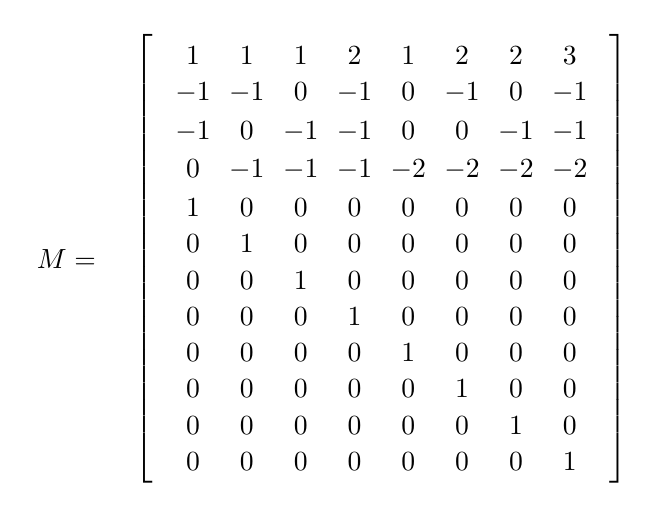
\begin{tikzpicture}

\node (G) {\( M = \)};

\matrix (M)
[matrix of math nodes,
 right of = G,
 xshift = 3cm,
 ampersand replacement = \&,
 left delimiter = \lbrack,
 right delimiter = \rbrack]
{
1 \& 1 \& 1 \& 2 \& 1 \& 2 \& 2 \& 3 \\
-1 \& -1 \& 0 \& -1 \& 0 \& -1 \& 0 \& -1 \\
-1 \& 0 \& -1 \& -1 \& 0 \& 0 \& -1 \& -1 \\
0 \& -1 \& -1 \& -1 \& -2 \& -2 \& -2 \& -2 \\
1 \& 0 \& 0 \& 0 \& 0 \& 0 \& 0 \& 0 \\
0 \& 1 \& 0 \& 0 \& 0 \& 0 \& 0 \& 0 \\
0 \& 0 \& 1 \& 0 \& 0 \& 0 \& 0 \& 0 \\
0 \& 0 \& 0 \& 1 \& 0 \& 0 \& 0 \& 0 \\
0 \& 0 \& 0 \& 0 \& 1 \& 0 \& 0 \& 0 \\
0 \& 0 \& 0 \& 0 \& 0 \& 1 \& 0 \& 0 \\
0 \& 0 \& 0 \& 0 \& 0 \& 0 \& 1 \& 0 \\
0 \& 0 \& 0 \& 0 \& 0 \& 0 \& 0 \& 1 \\
};

\end{tikzpicture}
}
\subfigure[Minor to calculate determinant of, with columns and rows eliminated
by Laplace expansion marked.]{
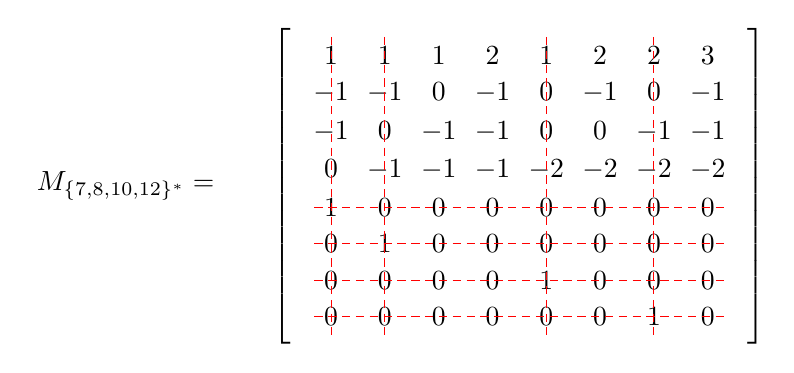
\begin{tikzpicture}

\node[xshift = -5cm] (G1) {\( M_{\{7, 8, 10, 12\}^*} = \)};

\matrix (M)
[matrix of math nodes,
 right of = G1,
 xshift = 4cm,
 ampersand replacement = \&,
 left delimiter = \lbrack,
 right delimiter = \rbrack]
{
1 \& 1 \& 1 \& 2 \& 1 \& 2 \& 2 \& 3 \\
-1 \& -1 \& 0 \& -1 \& 0 \& -1 \& 0 \& -1 \\
-1 \& 0 \& -1 \& -1 \& 0 \& 0 \& -1 \& -1 \\
0 \& -1 \& -1 \& -1 \& -2 \& -2 \& -2 \& -2 \\
1 \& 0 \& 0 \& 0 \& 0 \& 0 \& 0 \& 0 \\
0 \& 1 \& 0 \& 0 \& 0 \& 0 \& 0 \& 0 \\
0 \& 0 \& 0 \& 0 \& 1 \& 0 \& 0 \& 0 \\
0 \& 0 \& 0 \& 0 \& 0 \& 0 \& 1 \& 0 \\
};

\draw[red, densely dashed] (M-5-1.west) to (M-5-8.east);
\draw[red, densely dashed] (M-1-1.north) to (M-8-1.south);
\draw[red, densely dashed] (M-6-1.west) to (M-6-8.east);
\draw[red, densely dashed] (M-1-2.north) to (M-8-2.south);
\draw[red, densely dashed] (M-7-1.west) to (M-7-8.east);
\draw[red, densely dashed] (M-1-5.north) to (M-8-5.south);
\draw[red, densely dashed] (M-8-1.west) to (M-8-8.east);
\draw[red, densely dashed] (M-1-7.north) to (M-8-7.south);

\end{tikzpicture}
}

\caption{Illustration of how to calculate Grassmann coordinates}

\end{figure}

If we choose to invent som strange notation to represent the matrix with those
elements we might say that
\[
	S_{u \times u} = S_{\mathcal{U}, \{i_m - 4 | i_m \in \mathcal{L}\}^*},
\]
where the star means we take the complement with respect to all possible indices.

Putting it all together we will thus have that
\[
	a_{i_1 \cdots i_{4(k-1)}} =
	(-1)^{\lceil \frac{u}{2} \rceil} \cdot \prod_{m = u + 1}^{4(k-1)} (-1)^{i_m} \cdot
	|S_{\mathcal{U}, \{i_m - 4 | i_m \in \mathcal{L}\}^*}|
\]

To be more concrete, let us say that \( \{i_m - 4 | i_m \in \mathcal{L}\}^* =
\{j_1, j_2, j_3, j_4\} \). By the division algorithm we can write
\( j_t = 4 \cdot \alpha_t + \beta_t \). So for the four cases of \( \beta_t \) the columns where the
elements of the determinant part will be
\[
	\begin{matrix}
		\beta_t = 0 & \beta_t = 1 & \beta_t = 2 & \beta_t = 3 \\
		& & & \\
		\begin{bmatrix}
			\alpha_t - 1 \\ 0 \\ 0 \\ -\alpha_t
		\end{bmatrix} & \begin{bmatrix}
			\alpha_t \\ -1 \\ 0 \\ -\alpha_t
		\end{bmatrix} & \begin{bmatrix}
			\alpha_t \\ 0 \\ -1 \\ -\alpha_t
		\end{bmatrix} & \begin{bmatrix}
			\alpha_t + 1 \\ -1 \\ -1 \\ -\alpha_t
		\end{bmatrix}
	\end{matrix}.
\]
We will make a table, so that given the four indices with the division algorithm applied to them
we can immidiatly say what the Grassmann coordinate will be.
\begin{longtable}{|l|l|l|l|l|l|}
0 0 0 0 & \(0\) & 1 1 1 2 & \(0\) & 2 2 3 0 & \(\alpha_2 - \alpha_3\) \\ 
0 0 0 1 & \(0\) & 1 1 1 3 & \(0\) & 2 2 3 1 & \(\alpha_2 - \alpha_3\) \\ 
0 0 0 2 & \(0\) & 1 1 2 0 & \(\alpha_3 - \alpha_2\) & 2 2 3 2 & \(0\) \\ 
0 0 0 3 & \(0\) & 1 1 2 1 & \(0\) & 2 2 3 3 & \(0\) \\ 
0 0 1 0 & \(0\) & 1 1 2 2 & \(0\) & 2 3 0 0 & \(\alpha_4 - \alpha_1\) \\ 
0 0 1 1 & \(0\) & 1 1 2 3 & \(\alpha_2 - \alpha_3\) & 2 3 0 1 & \(\alpha_3 + \alpha_4 - \alpha_1 - \alpha_2\) \\ 
0 0 1 2 & \(\alpha_3 - \alpha_2\) & 1 1 3 0 & \(\alpha_3 - \alpha_2\) & 2 3 0 2 & \(\alpha_2 - \alpha_1\) \\ 
0 0 1 3 & \(\alpha_3 - \alpha_2\) & 1 1 3 1 & \(0\) & 2 3 0 3 & \(\alpha_3 - \alpha_1\) \\ 
0 0 2 0 & \(0\) & 1 1 3 2 & \(\alpha_3 - \alpha_2\) & 2 3 1 0 & \(\alpha_2 + \alpha_4 - \alpha_1 - \alpha_3\) \\ 
0 0 2 1 & \(\alpha_2 - \alpha_3\) & 1 1 3 3 & \(0\) & 2 3 1 1 & \(\alpha_4 - \alpha_1\) \\ 
0 0 2 2 & \(0\) & 1 2 0 0 & \(\alpha_1 - \alpha_4\) & 2 3 1 2 & \(\alpha_2 - \alpha_1\) \\ 
0 0 2 3 & \(\alpha_2 - \alpha_3\) & 1 2 0 1 & \(\alpha_1 - \alpha_2\) & 2 3 1 3 & \(\alpha_3 - \alpha_1\) \\ 
0 0 3 0 & \(0\) & 1 2 0 2 & \(\alpha_1 - \alpha_3\) & 2 3 2 0 & \(\alpha_4 - \alpha_2\) \\ 
0 0 3 1 & \(\alpha_2 - \alpha_3\) & 1 2 0 3 & \(\alpha_1 + \alpha_4 - \alpha_2 - \alpha_3\) & 2 3 2 1 & \(\alpha_4 - \alpha_2\) \\ 
0 0 3 2 & \(\alpha_3 - \alpha_2\) & 1 2 1 0 & \(\alpha_2 - \alpha_4\) & 2 3 2 2 & \(0\) \\ 
0 0 3 3 & \(0\) & 1 2 1 1 & \(0\) & 2 3 2 3 & \(0\) \\ 
0 1 0 0 & \(0\) & 1 2 1 2 & \(0\) & 2 3 3 0 & \(\alpha_4 - \alpha_3\) \\ 
0 1 0 1 & \(0\) & 1 2 1 3 & \(\alpha_4 - \alpha_2\) & 2 3 3 1 & \(\alpha_4 - \alpha_3\) \\ 
0 1 0 2 & \(\alpha_2 - \alpha_4\) & 1 2 2 0 & \(\alpha_3 - \alpha_4\) & 2 3 3 2 & \(0\) \\ 
0 1 0 3 & \(\alpha_2 - \alpha_4\) & 1 2 2 1 & \(0\) & 2 3 3 3 & \(0\) \\ 
0 1 1 0 & \(0\) & 1 2 2 2 & \(0\) & 3 0 0 0 & \(0\) \\ 
0 1 1 1 & \(0\) & 1 2 2 3 & \(\alpha_4 - \alpha_3\) & 3 0 0 1 & \(\alpha_3 - \alpha_4\) \\ 
0 1 1 2 & \(\alpha_3 - \alpha_4\) & 1 2 3 0 & \(\alpha_2 + \alpha_3 - \alpha_1 - \alpha_4\) & 3 0 0 2 & \(\alpha_4 - \alpha_3\) \\ 
0 1 1 3 & \(\alpha_3 - \alpha_4\) & 1 2 3 1 & \(\alpha_2 - \alpha_1\) & 3 0 0 3 & \(0\) \\ 
0 1 2 0 & \(\alpha_1 - \alpha_2\) & 1 2 3 2 & \(\alpha_3 - \alpha_1\) & 3 0 1 0 & \(\alpha_1 - \alpha_3\) \\ 
0 1 2 1 & \(\alpha_1 - \alpha_3\) & 1 2 3 3 & \(\alpha_4 - \alpha_1\) & 3 0 1 1 & \(\alpha_1 - \alpha_4\) \\ 
0 1 2 2 & \(\alpha_1 - \alpha_4\) & 1 3 0 0 & \(\alpha_1 - \alpha_4\) & 3 0 1 2 & \(\alpha_1 + \alpha_4 - \alpha_2 - \alpha_3\) \\ 
0 1 2 3 & \(\alpha_1 + \alpha_2 - \alpha_3 - \alpha_4\) & 1 3 0 1 & \(\alpha_1 - \alpha_2\) & 3 0 1 3 & \(\alpha_1 - \alpha_2\) \\ 
0 1 3 0 & \(\alpha_1 - \alpha_2\) & 1 3 0 2 & \(\alpha_1 + \alpha_2 - \alpha_3 - \alpha_4\) & 3 0 2 0 & \(\alpha_3 - \alpha_1\) \\ 
0 1 3 1 & \(\alpha_1 - \alpha_3\) & 1 3 0 3 & \(\alpha_1 - \alpha_3\) & 3 0 2 1 & \(\alpha_2 + \alpha_3 - \alpha_1 - \alpha_4\) \\ 
0 1 3 2 & \(\alpha_1 + \alpha_3 - \alpha_2 - \alpha_4\) & 1 3 1 0 & \(\alpha_2 - \alpha_4\) & 3 0 2 2 & \(\alpha_4 - \alpha_1\) \\ 
0 1 3 3 & \(\alpha_1 - \alpha_4\) & 1 3 1 1 & \(0\) & 3 0 2 3 & \(\alpha_2 - \alpha_1\) \\ 
0 2 0 0 & \(0\) & 1 3 1 2 & \(\alpha_2 - \alpha_4\) & 3 0 3 0 & \(0\) \\ 
0 2 0 1 & \(\alpha_4 - \alpha_2\) & 1 3 1 3 & \(0\) & 3 0 3 1 & \(\alpha_2 - \alpha_4\) \\ 
0 2 0 2 & \(0\) & 1 3 2 0 & \(\alpha_1 + \alpha_3 - \alpha_2 - \alpha_4\) & 3 0 3 2 & \(\alpha_4 - \alpha_2\) \\ 
0 2 0 3 & \(\alpha_4 - \alpha_2\) & 1 3 2 1 & \(\alpha_1 - \alpha_2\) & 3 0 3 3 & \(0\) \\ 
0 2 1 0 & \(\alpha_2 - \alpha_1\) & 1 3 2 2 & \(\alpha_1 - \alpha_4\) & 3 1 0 0 & \(\alpha_4 - \alpha_1\) \\ 
0 2 1 1 & \(\alpha_4 - \alpha_1\) & 1 3 2 3 & \(\alpha_1 - \alpha_3\) & 3 1 0 1 & \(\alpha_3 - \alpha_1\) \\ 
0 2 1 2 & \(\alpha_3 - \alpha_1\) & 1 3 3 0 & \(\alpha_3 - \alpha_4\) & 3 1 0 2 & \(\alpha_2 + \alpha_4 - \alpha_1 - \alpha_3\) \\ 
0 2 1 3 & \(\alpha_3 + \alpha_4 - \alpha_1 - \alpha_2\) & 1 3 3 1 & \(0\) & 3 1 0 3 & \(\alpha_2 - \alpha_1\) \\ 
0 2 2 0 & \(0\) & 1 3 3 2 & \(\alpha_3 - \alpha_4\) & 3 1 1 0 & \(\alpha_4 - \alpha_3\) \\ 
0 2 2 1 & \(\alpha_4 - \alpha_3\) & 1 3 3 3 & \(0\) & 3 1 1 1 & \(0\) \\ 
0 2 2 2 & \(0\) & 2 0 0 0 & \(0\) & 3 1 1 2 & \(\alpha_4 - \alpha_3\) \\ 
0 2 2 3 & \(\alpha_4 - \alpha_3\) & 2 0 0 1 & \(\alpha_3 - \alpha_4\) & 3 1 1 3 & \(0\) \\ 
0 2 3 0 & \(\alpha_2 - \alpha_1\) & 2 0 0 2 & \(0\) & 3 1 2 0 & \(\alpha_3 + \alpha_4 - \alpha_1 - \alpha_2\) \\ 
0 2 3 1 & \(\alpha_2 + \alpha_4 - \alpha_1 - \alpha_3\) & 2 0 0 3 & \(\alpha_3 - \alpha_4\) & 3 1 2 1 & \(\alpha_3 - \alpha_1\) \\ 
0 2 3 2 & \(\alpha_3 - \alpha_1\) & 2 0 1 0 & \(\alpha_1 - \alpha_3\) & 3 1 2 2 & \(\alpha_4 - \alpha_1\) \\ 
0 2 3 3 & \(\alpha_4 - \alpha_1\) & 2 0 1 1 & \(\alpha_1 - \alpha_4\) & 3 1 2 3 & \(\alpha_2 - \alpha_1\) \\ 
0 3 0 0 & \(0\) & 2 0 1 2 & \(\alpha_1 - \alpha_2\) & 3 1 3 0 & \(\alpha_4 - \alpha_2\) \\ 
0 3 0 1 & \(\alpha_4 - \alpha_2\) & 2 0 1 3 & \(\alpha_1 + \alpha_3 - \alpha_2 - \alpha_4\) & 3 1 3 1 & \(0\) \\ 
0 3 0 2 & \(\alpha_2 - \alpha_4\) & 2 0 2 0 & \(0\) & 3 1 3 2 & \(\alpha_4 - \alpha_2\) \\ 
0 3 0 3 & \(0\) & 2 0 2 1 & \(\alpha_2 - \alpha_4\) & 3 1 3 3 & \(0\) \\ 
0 3 1 0 & \(\alpha_2 - \alpha_1\) & 2 0 2 2 & \(0\) & 3 2 0 0 & \(\alpha_1 - \alpha_4\) \\ 
0 3 1 1 & \(\alpha_4 - \alpha_1\) & 2 0 2 3 & \(\alpha_2 - \alpha_4\) & 3 2 0 1 & \(\alpha_1 + \alpha_3 - \alpha_2 - \alpha_4\) \\ 
0 3 1 2 & \(\alpha_2 + \alpha_3 - \alpha_1 - \alpha_4\) & 2 0 3 0 & \(\alpha_1 - \alpha_3\) & 3 2 0 2 & \(\alpha_1 - \alpha_3\) \\ 
0 3 1 3 & \(\alpha_3 - \alpha_1\) & 2 0 3 1 & \(\alpha_1 + \alpha_2 - \alpha_3 - \alpha_4\) & 3 2 0 3 & \(\alpha_1 - \alpha_2\) \\ 
0 3 2 0 & \(\alpha_1 - \alpha_2\) & 2 0 3 2 & \(\alpha_1 - \alpha_2\) & 3 2 1 0 & \(\alpha_1 + \alpha_2 - \alpha_3 - \alpha_4\) \\ 
0 3 2 1 & \(\alpha_1 + \alpha_4 - \alpha_2 - \alpha_3\) & 2 0 3 3 & \(\alpha_1 - \alpha_4\) & 3 2 1 1 & \(\alpha_1 - \alpha_4\) \\ 
0 3 2 2 & \(\alpha_1 - \alpha_4\) & 2 1 0 0 & \(\alpha_4 - \alpha_1\) & 3 2 1 2 & \(\alpha_1 - \alpha_3\) \\ 
0 3 2 3 & \(\alpha_1 - \alpha_3\) & 2 1 0 1 & \(\alpha_3 - \alpha_1\) & 3 2 1 3 & \(\alpha_1 - \alpha_2\) \\ 
0 3 3 0 & \(0\) & 2 1 0 2 & \(\alpha_2 - \alpha_1\) & 3 2 2 0 & \(\alpha_3 - \alpha_4\) \\ 
0 3 3 1 & \(\alpha_4 - \alpha_3\) & 2 1 0 3 & \(\alpha_2 + \alpha_3 - \alpha_1 - \alpha_4\) & 3 2 2 1 & \(\alpha_3 - \alpha_4\) \\ 
0 3 3 2 & \(\alpha_3 - \alpha_4\) & 2 1 1 0 & \(\alpha_4 - \alpha_3\) & 3 2 2 2 & \(0\) \\ 
0 3 3 3 & \(0\) & 2 1 1 1 & \(0\) & 3 2 2 3 & \(0\) \\ 
1 0 0 0 & \(0\) & 2 1 1 2 & \(0\) & 3 2 3 0 & \(\alpha_2 - \alpha_4\) \\ 
1 0 0 1 & \(0\) & 2 1 1 3 & \(\alpha_3 - \alpha_4\) & 3 2 3 1 & \(\alpha_2 - \alpha_4\) \\ 
1 0 0 2 & \(\alpha_4 - \alpha_3\) & 2 1 2 0 & \(\alpha_4 - \alpha_2\) & 3 2 3 2 & \(0\) \\ 
1 0 0 3 & \(\alpha_4 - \alpha_3\) & 2 1 2 1 & \(0\) & 3 2 3 3 & \(0\) \\ 
1 0 1 0 & \(0\) & 2 1 2 2 & \(0\) & 3 3 0 0 & \(0\) \\ 
1 0 1 1 & \(0\) & 2 1 2 3 & \(\alpha_2 - \alpha_4\) & 3 3 0 1 & \(\alpha_3 - \alpha_2\) \\ 
1 0 1 2 & \(\alpha_4 - \alpha_2\) & 2 1 3 0 & \(\alpha_1 + \alpha_4 - \alpha_2 - \alpha_3\) & 3 3 0 2 & \(\alpha_2 - \alpha_3\) \\ 
1 0 1 3 & \(\alpha_4 - \alpha_2\) & 2 1 3 1 & \(\alpha_1 - \alpha_3\) & 3 3 0 3 & \(0\) \\ 
1 0 2 0 & \(\alpha_3 - \alpha_1\) & 2 1 3 2 & \(\alpha_1 - \alpha_2\) & 3 3 1 0 & \(\alpha_2 - \alpha_3\) \\ 
1 0 2 1 & \(\alpha_2 - \alpha_1\) & 2 1 3 3 & \(\alpha_1 - \alpha_4\) & 3 3 1 1 & \(0\) \\ 
1 0 2 2 & \(\alpha_4 - \alpha_1\) & 2 2 0 0 & \(0\) & 3 3 1 2 & \(\alpha_2 - \alpha_3\) \\ 
1 0 2 3 & \(\alpha_2 + \alpha_4 - \alpha_1 - \alpha_3\) & 2 2 0 1 & \(\alpha_3 - \alpha_2\) & 3 3 1 3 & \(0\) \\ 
1 0 3 0 & \(\alpha_3 - \alpha_1\) & 2 2 0 2 & \(0\) & 3 3 2 0 & \(\alpha_3 - \alpha_2\) \\ 
1 0 3 1 & \(\alpha_2 - \alpha_1\) & 2 2 0 3 & \(\alpha_3 - \alpha_2\) & 3 3 2 1 & \(\alpha_3 - \alpha_2\) \\ 
1 0 3 2 & \(\alpha_3 + \alpha_4 - \alpha_1 - \alpha_2\) & 2 2 1 0 & \(\alpha_2 - \alpha_3\) & 3 3 2 2 & \(0\) \\ 
1 0 3 3 & \(\alpha_4 - \alpha_1\) & 2 2 1 1 & \(0\) & 3 3 2 3 & \(0\) \\ 
1 1 0 0 & \(0\) & 2 2 1 2 & \(0\) & 3 3 3 0 & \(0\) \\ 
1 1 0 1 & \(0\) & 2 2 1 3 & \(\alpha_3 - \alpha_2\) & 3 3 3 1 & \(0\) \\ 
1 1 0 2 & \(\alpha_2 - \alpha_3\) & 2 2 2 0 & \(0\) & 3 3 3 2 & \(0\) \\ 
1 1 0 3 & \(\alpha_2 - \alpha_3\) & 2 2 2 1 & \(0\) & 3 3 3 3 & \(0\) \\ 
1 1 1 0 & \(0\) & 2 2 2 2 & \(0\) & 0 0 0 0 & \(0\) \\ 
1 1 1 1 & \(0\) & 2 2 2 3 & \(0\) & 0 0 0 0 & \(0\) \\ 
\end{longtable}

Since Grassmann coordinates are invariant under affine transformations, this \emph{tube} will have
the same coordinates irregardless of whether we do a coordinate change to switch axis it follows.
Or if we morph it in any way that preserves parallellism. A skew tube will be equivalent to this
straight tube.

\subsubsection{Cubic grid} % (fold)
\label{ssub:cubic_grid}
Let us now move further by considering a complete grid in \( \mathbb{R}^3 \), basically by stacking
the tubes considered above.
\begin{figure}
\begin{center}
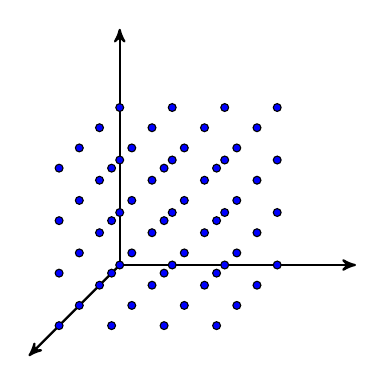
\begin{tikzpicture}[scale=2, auto, >=stealth']

\draw[->,thick] (0,0,0) -- (1.5,0,0);
\draw[->,thick] (0,0,0) -- (0,1.5,0);
\draw[->,thick] (0,0,0) -- (0,0,1.5);

\foreach \x in {0,1/3,2/3,3/3}
{
	\foreach \y in {0,1/3,2/3,3/3}
	{
		\foreach \z in {0,1/3,2/3,3/3}
		{
			\node at (\x,\y,\z) [circle,inner sep=0pt,minimum size=1mm,fill=blue,draw=black] {};
		}
	}
}

\end{tikzpicture}
\end{center}
\end{figure}

The S-matrix for the shape space spanned by the cubic grid will be
\[
	\begin{bmatrix}
		\begin{matrix}
			A_0 & A_1 & \cdots & A_{n-1}
		\end{matrix} \\
		I
	\end{bmatrix},
\]
where every \( A_k \) is of the form
\[
	A_k = \begin{bmatrix}
		\begin{matrix}
			B_0 & B_1 & \cdots & B_{n - 1}
		\end{matrix} \\
		\begin{matrix}
			-k & \cdots & -k
		\end{matrix}
	\end{bmatrix},
\]
and further, every \( B_l \) is of the form
\[
	B_l = \begin{bmatrix}
		k + l - 1 & k - l & \cdots & k + l + n - 2 \\
		0 & -1 & \cdots & -(n-1) \\
		-l & -l & \cdots & -l
	\end{bmatrix}
\]
with the special cases
\[
	B_0 = \begin{bmatrix}
		1 & 2 & 3 & 4 \\
		-2 & -3 & -4 & -5 \\
		0 & 0 & 0 & 0
	\end{bmatrix}
\]
and
\[
	B_1 = \begin{bmatrix}
		1 & 2 & 3 & 4 & 5\\
		-1 & -2 & -3 & -4 & -5 \\
		-1 & -1 & -1 & -1 & -1
	\end{bmatrix}
\]
inside the \( A_0 \) block.
As we did above, when calculating a Grassmann coordinate, in stead of considering the indices which
represents the rows chosen in the S-matrix we look at the rows \emph{not} chosen. As we saw above,
this will give the columns in the \( 4 \times 4 \) matrix whose determinant will give the value
of the coordinate up to sign. Let \( s_i \) be one of the four indices. The column determined by
this index which will be part of the \( 4 \times 4 \) matrix can be found by looking at
\[
	s_i = a_i \cdot n^2 + b_i \cdot n + c_i.
\]
This will mean \( s_i \) represents the \( c_i \)'th column of the block \( B_{b_i} \) within
\( A_{a_i} \), namely
\[
	\begin{bmatrix}
		a_i + b_i + c_i - 1 \\ -c_i \\ -b_i \\ -a_i
	\end{bmatrix}.
\]
So the coordinate \( a_{s_1 s_2 s_3 s_4} \) will be
\[
	a_{s_1 s_2 s_3 s_4} = s \cdot \begin{vmatrix}
		a_1 + b_1 + c_1 - 1 & \cdots & a_4 + b_4 + c_4 - 1 \\
		-c_1 & \cdots & -c_4 \\
		-b_1 & \cdots & -b_4 \\
		-a_1 & \cdots & -a_4 \\
	\end{vmatrix},
\]
where \( s \) is the sign.

\begin{Example}
	We make cubic grid with resolution \( 9 \), for this there will be 
	\( {9^3 \choose 4} = {729 \choose 4} = 11 671 285 626 \) coordinates. Let
	us calculate the coordinate \( \alpha_{\{25, 411, 286, 412\}^*} \).
	We will need to factor the indices in to the form 
	\( a \cdot 27 + b \cdot 9 + c \);
	\begin{align*}
		25 &= 0 \cdot 27 + 2 \cdot 9 + 7, \\
		411 &= 15 \cdot 27 + 0 \cdot 9 + 6,\\
		286 &= 10 \cdot 27 + 1 \cdot 9 + 7,\\
		412 &= 15 \cdot 27 + 0 \cdot 9 + 7.\\
	\end{align*}
	Thus we need to calculate the determinant
	\[
		\begin{vmatrix}
			0 + 2 + 7 - 1 & 15 + 0 + 9 - 1 & 10 + 1 + 7 - 1 & 15 + 0 + 7 - 1 \\
			-7 & -6 & -7 & -7 \\
			-2 & 0 & -1 & 0 \\
			-15 & -10 & -15 & 0
		\end{vmatrix} =
	\]
	\[
		\begin{vmatrix}
			8 & 23 & 17 & 21 \\
			-7 & -6 & -7 & -7 \\
			-2 & 0 & -1 & 0 \\
			-15 & -10 & -15 & 0
		\end{vmatrix}.
	\]
	We utilize the condensation method to calculate this.
	\[
		\begin{bmatrix}
			-2  &   0 &  -1 &   0 \\
			 8  &  23 &  17 &  21 \\
			-7  &  -6 &  -7 &  -7 \\
			-15 & -10 & -15 &   0
		\end{bmatrix}
	\]
	\[
		\begin{bmatrix}
			\begin{vmatrix}
				-2 & 0 \\ 8 & 23
			\end{vmatrix} & \begin{vmatrix}
				0 & -1 \\ 23 & 17
			\end{vmatrix} & \begin{vmatrix}
				-1 & 17 \\ 0 & 21
			\end{vmatrix} \\ & & \\ \begin{vmatrix}
				8 & 23 \\ -7 & -6
			\end{vmatrix} & \begin{vmatrix}
				23 & 17 \\ -6 & -7
			\end{vmatrix} & \begin{vmatrix}
				17 & 21 \\ -7 & -7
			\end{vmatrix} \\ & & \\ \begin{vmatrix}
				-7 & -6 \\ -15 & -10
			\end{vmatrix} & \begin{vmatrix}
				-6 & -7 \\ -10 & -15
			\end{vmatrix} & \begin{vmatrix}
				-7 & -7 \\ -15 & 0
			\end{vmatrix}
		\end{bmatrix} = \begin{bmatrix}
			-46 & 23 & -21 \\
			113 & -59 & 28 \\
			-20 & 20 & -105
		\end{bmatrix}
	\]
	\[
		\begin{bmatrix}
			\frac{\begin{vmatrix}
				-46 & 23 \\ 113 & -59
			\end{vmatrix}}{23} & \frac{\begin{vmatrix}
				23 & -21 \\ -59 & 28
			\end{vmatrix}}{17} \\ & \\ \frac{\begin{vmatrix}
				113 & -59 \\ -20 & 20
			\end{vmatrix}}{-6} & \frac{\begin{vmatrix}
				-59 & 28 \\ 20 & -105
			\end{vmatrix}}{-7}
		\end{bmatrix} = \begin{bmatrix}
			5 & -35 \\ -180 & -805
		\end{bmatrix}
	\]
	\[
		\frac{\begin{vmatrix}
			5 & -35 \\ -180 & -805
		\end{vmatrix}}{-59} = 175
	\]
	Thus \( \alpha_{\{25, 411, 286, 412\}^*} = s \cdot 175 \), so what is
	\( s \)? Since the numbers \( \{1,2,3,4\} \) is part of the selected set
	we have
	\[
		s = \prod_{j = 4}^{725} (-1)^{i_j + i_j + 4} = 
		\left(\prod_{j = 4}^{725} (-1)^{i_j}\right)^2 = 1.
	\]
\end{Example}

% subsubsection cubic_grid (end)

\subsubsection{Tube with varied length and resolution} % (fold)
We can vary the length of the grid (or tube) in one direction, while also
varying \emph{width} of the tube (so that two of the sides of the 
regular spatial grid will be the same).

Say we have length \( k \) and ``width" or ``resolution" \( l \), then the
S-matrix will just as above consist of \( k \) \( A \)-blocks. However, every
\( A_i \) will consist of \( l \) \( B \)-blocks of the form
\[
	B_j(i) = \begin{bmatrix}
		i + j - 2 & i + 1 + j - 2 & \cdots & i + l - 1 + j - 2 & i + l + j - 2 \\
		0 & -1 & \cdots & -l + 2 & -l + 1 \\
		-j & -j & \cdots & -j & -j \\
		-i & -i & \cdots & -i & -i
	\end{bmatrix}.
\]
We do however have a few special cases; both in \( A_0 \) and \( A_1 \).
In \( A_0 \) we have
\[
	B_0(0) = \begin{bmatrix}
		1 & 2 & \cdots & l - 2 \\
		-2 & -3 & \cdots & -l + 1 \\
		0 & 0 & \cdots & 0 \\
		0 & 0 & \cdots & 0
	\end{bmatrix}, 
	B_1(0) = \begin{bmatrix}
		1 & 2 & \cdots & l - 1 \\
		-1 & -2 & \cdots & -l + 1 \\
		-1 & -1 & \cdots & -1 \\
		0 & 0 & \cdots & 0
	\end{bmatrix}
\]
and in \( A_1 \) we have
\[
	B_0(1) = \begin{bmatrix}
		1 & 2 & \cdots & l - 1 \\
		-1 & -2 & \cdots & -l + 1 \\
		0 & 0 & \cdots & 0 \\
		-1 & -1 & \cdots & -1
	\end{bmatrix}.
\]
Note also that these three blocks are smaller than the other \( B \)-blocks,
\( B_0(0) \) is two columns shorter, and \( B_0(1), B_1(0) \) have one less
column.

We now have the information we need in order to do the same calculations as we
did for the cubic grid in order to obtain an expression for the Grassmann
coordinates. But let us refrain from this and move straight in to the more
general case in the next section.

\subsubsection{Parallelepiped with arbitrary resolution in any direction}
Now we consider a box in three dimensional space with independant height,
width, and depth. These we can say are the elements of the triple 
\( k, l, m \). Due to affine invariance, we can assume that \( k < l < m \);
would it be any other way we could simply transform the shape in to this form
by a rotation and a translation.
We will then have an \( S \)-matrix consisting of \( k \) \( A \)-blocks,
each of which in turn will consist of \( l \) \( B \)-blocks. Beside special
cases for the first \( B \)-blocks in the first \( A \)-blocks, a \( B \)-block
will be of shape \( m \times 4 \). Let us write it out.
\[
	S = \begin{bmatrix}
		\begin{matrix}
			A_0 & A_1 & \cdots & A_{k - 1}
		\end{matrix} \\
		I
	\end{bmatrix},
\]
where
\[
	A_i = \begin{bmatrix}
		B_0(i) & B_1(i) & \cdots & B_{l - 1}(i)
	\end{bmatrix};
\]
where in turn
\[
	B_j(i) = \begin{bmatrix}
		i - 2 + j & i - 1 + j & \cdots & i - 2 + m + j & i - 1 + m + j \\
		0 & -1 & \cdots & -m + 2 & -m + 1 \\
		-j & -j & \cdots & -j & -j \\
		-i + 1 & -i + 1 & \cdots & -i + 1 & -i + 1
	\end{bmatrix}.
\]
Of course, there are the special cases,
\[
	B_0(0) = \begin{bmatrix}
		1 & 2 & \cdots & m - 3 & m - 2 \\
		-2 & -3 & \cdots & -m + 2 & -m + 1 \\
		0 & 0 & \cdots & 0 & 0 \\
		0 & 0 & \cdots & 0 & 0
	\end{bmatrix},
	B_1(0) = \begin{bmatrix}
		1 & 2 & \cdots & m - 2 & m - 1 \\
		-1 & -2 & \cdots & -m + 2 & -m + 1 \\
		-1 & -1 & \cdots & -1 & -1 \\
		0 & 0 & \cdots & 0 & 0
	\end{bmatrix},
\]
\[
	B_0(1) = \begin{bmatrix}
		1 & 2 & \cdots & m - 2 & m - 1 \\
		-1 & -2 & \cdots & -m + 2 & -m + 1 \\
		0 & 0 & \cdots & 0 & 0 \\
		-1 & -1 & \cdots & -1 & -1
\end{bmatrix}.
\]
Let us perform the same reaasoning as we did for the cubic grid a few 
pages ago with
the goal to find an expression for an arbitrary Grassmann coordinate.

We look at the Grassmann coordinate where the index is the complement of
\( \{s_1, s_2, s_3, s_4\} \), and call it \( \alpha_{s_1 s_2 s_3 s_4} \).
As per above we can say that \( s_i \) represents the \( c_i \)'th column
of the block \( B_{b_i} \) within block \( A_{a_i} \) (starting from zero), 
which we can partition
as
\[
	s_i = a_i \cdot l \cdot m + b_i \cdot m + c_i.
\]
Using this fomrulation, we can write the specified column as
\[
	\begin{bmatrix}
		a_i + b_i + c_i - 2\\
		-c_i\\
		-b_i \\
		-a_i + 1
	\end{bmatrix}
\]
Thus for the Grassmann coordinate \( \alpha_{s_1 s_2 s_3 s_4} \) we have
the expression
\[
	\alpha_{s_1 s_2 s_3 s_4} = s \cdot \begin{vmatrix}
		a_1 + b_1 + c_1 - 2 & a_2 + b_2 + c_2 - 2 & a_3 + b_3 + c_3 - 2 & 
		a_4 + b_4 + c_4 - 2 \\
		-c_1 & -c_2 & -c_3 & -c_4 \\
		-b_1 & -b_2 & -b_3 & -b_4 \\
		-a_1 + 1 & -a_2 + 1 & -a_3 + 1 & -a_4 + 1
	\end{vmatrix},
\]
where \( s \) is the sign.

\begin{Example}
	As for the cubic grid, let us make this more concrete by calculating a
	Grassmann coordinate. We make a grid with resolution \( (13, 8, 5) \), the
	shape space of this grid will be spanned by an S-matrix of size
	\( (13 \cdot 8 \cdot 5 = 520) \times (520 - 4 = 516)  \). We will in total
	for this shape space have \( {520 \choose 516} = 3 011 478 470 \)
	Grassmann coordinates. We will calculate the coordinate
	\( \alpha_{\{45, 195, 187, 36\}^*} \). First we partition the indexes;
	\begin{align*}
		45 &= 1 \cdot 40 + 1 \cdot 5 + 0, \\
		195 &= 4 \cdot 40 + 7 \cdot 5 + 0, \\
		187 &= 4 \cdot 40 + 5 \cdot 5 + 2, \\
		36 &= 0 \cdot 40 + 7 \cdot 5 + 1.
	\end{align*}
	So we shall calculate the determinant
	\[
		\begin{vmatrix}
			1 + 1 + 0 -2 & 4 + 7 + 0 - 2 & 4 + 5 + 2 - 2 & 0 + 7 + 5 - 1 - 2 \\
			0 & 0 & -2 & -1 \\
			-1 & -7 & -5 & -7 \\
			-1 + 1 & -4 + 1 & -4 + 1 & 0 + 1
		\end{vmatrix}		
	\]
	\[
		\begin{vmatrix}
			0 & 9 & 9 & 9 \\
			0 & 0 & -2 & -1 \\
			-1 & -7 & -5 & -7 \\
			0 & -3 & -3 & 1
		\end{vmatrix} =
		\begin{vmatrix}
			0 & 0 & -2 & -1 \\
			0 & 9 & 9 & 9 \\
			-1 & -7 & -5 & -7 \\
			0 & -3 & -3 & 1
		\end{vmatrix}	
	\]
	\[
		\begin{bmatrix}
			\begin{vmatrix}
				0 & 0 \\ 0 & 9
			\end{vmatrix} & \begin{vmatrix}
				0 & -2 \\ 9 & 9
			\end{vmatrix} & \begin{vmatrix}
				-2 & -1 \\ 9 & 9
			\end{vmatrix} \\ & & \\ \begin{vmatrix}
				0 & 9 \\ -1 & -7
			\end{vmatrix} & \begin{vmatrix}
				9 & 9 \\ -7 & -5
			\end{vmatrix} & \begin{vmatrix}
				9 & 9 \\ -5 & -7
			\end{vmatrix} \\ & & \\ \begin{vmatrix}
				-1 & -7 \\ 0 & -3
			\end{vmatrix} & \begin{vmatrix}
				-7 & -5 \\ -3 & -3
			\end{vmatrix} & \begin{vmatrix}
				-5 & -7 \\ -3 & 1
			\end{vmatrix}
		\end{bmatrix} = \begin{bmatrix}
			0 & 18 & -9 \\
			9 & 18 & -18 \\
			-3 & 6 & -26
		\end{bmatrix}
	\]
	\[
		\begin{bmatrix}
			\frac{\begin{vmatrix}
				0 & 18 \\ 9 & 18
			\end{vmatrix}}{9} & \frac{\begin{vmatrix}
				18 & -9 \\ 18 & -18
			\end{vmatrix}}{9} \\ & \\ \frac{\begin{vmatrix}
				9 & 18 \\ -3 & 6
			\end{vmatrix}}{-7} & \frac{\begin{vmatrix}
				18 & -18 \\ 6 & -26
			\end{vmatrix}}{-5}
		\end{bmatrix} = \begin{bmatrix}
			18 & -18 \\ \frac{-108}{7} & 72
		\end{bmatrix}
	\]
	\[
		\frac{\begin{bmatrix}
			18 & -18 \\ \frac{-108}{7} & 72
		\end{bmatrix}}{18} = \frac{396}{7}
	\]
	And the sign \( s \), will by the logic as above, be \( +1 \).
	So \( \alpha_{\{45, 195, 187, 36\}^*} = \frac{396}{7} \)
\end{Example}

% section using_grassmann_algebra_to_study_shape_space (end)

\chapter{Grassmann tensors} % (fold)
\label{sec:grassmann_tensors}

Say we have projection matrices
\( P^i : \mathbb{P}^n \to \mathbb{P}^{m_i} \).
From those we create
\[ P_{(-\sigma_1, -\sigma_2, \ldots )} =
\begin{bmatrix}
	P_{-\sigma_1}^1 \\
	P_{-\sigma_2}^2 \\
	P_{-\sigma_3}^3 \\
	\vdots
\end{bmatrix}.
\]
Note that each \( \sigma_i \) is an ordered sequence of integers in the range
\( 1, \ldots, m_i + 1 \).
The multidimensional array (indexed over sequences)
\[
	\mathcal{G}_{(-\sigma_1, -\sigma_2,\ldots)} =
	\text{sign}(\sigma_1) \cdot \text{sign}(\sigma_2) \cdot \ldots \cdot
	|P_{(-\sigma_1, -\sigma_2, \ldots )} |
\]
is the Grassmann tensor.

Say we have a number of points in some projecive space. These points will
span a linear subspace. If we were to put those points as columns in a matrix,
the column span would be that subspace. Let us call that matrix \( S \).
Any point in the span of \( S \) can be written as \( S v \), where \( v \)
is some vector.

Let a point \( X \in \mathbb{P}^n \) be projected by \( P^1 \) in to the
linear subspace \( span(S) \subset \mathbb{P}^{m_1}  \). That means there
exist a vector \( v \) such that
\[
	P^1 X - S v = 0.
\]
Keeping the point \( X \) fixed, but repeating the argument for every projection
we have, we get the relation
\[
	\begin{bmatrix}
		P^1 & S^1 & & & \\
		P^2 & & S^2 & & \\
		\vdots & & & \ddots & \\
	\end{bmatrix}
	\begin{bmatrix}
		X \\ -v_1 \\ -v_2 \\ \vdots
	\end{bmatrix} = 0.
\]
Let us count the rows and columns of that matrix.
We can immediately see that the number of rows is \( \sum_i (m_i + 1) \).
The number of columns depend on the number of points that span the subspaces \( S^i \).
Say that the subspace \( S^i \) is spanned by \( m_i + 1 - \alpha_i \) points, so that
\( \alpha_i \) will be the codimension of \( span(S^i) \subset \mathbb{P}^{m_i} \).
Then we will have \( n + 1 + \sum_i (m_i + 1 - \alpha_i) \) columns.
This means the matrix will be square exactly when \( \sum_i \alpha_i = n + 1 \), and then we
can calculate its determinant.

If we use the formula (\ref{eq:detformula}) we can calculate the determinant of
the matrix above as
\[
	\sum_{\sigma_1, \sigma_2, \cdots} \text{sign}(\sigma_1) \cdot \text{sign}(\sigma_2)
	\cdot \ldots \cdot |P_{(-\sigma_1, -\sigma_2, \ldots )} | \cdot
	|S_{\sigma_1}^1| \cdot |S_{\sigma_2}^2| \cdot \ldots .
\]
In that sum we have the elements of the Grassmann tensor. And as we want a linear dependence
between the subspaces \( S^i \), the determinant should be zero. So from the Grassmann tensor
we get a linear relation between the subspaces by
\[
	\sum_{\sigma_1, \sigma_2, \cdots} \mathcal{G}_{(-\sigma_1, -\sigma_2,\ldots)}
	\cdot |S_{\sigma_1}^1| \cdot |S_{\sigma_2}^2| \cdot \ldots = 0.
\]

Let us note that the requirement of \( \sum_i \alpha_i = n + 1 \) give some restrictions on
the subspaces for us to have the linear relation. For example, when \( n \) is fixed, as the
number of different projections increase, the codimensions of the subspaces must decrease.

Since the sequence \( (\alpha_1, \ldots ) \) is important to the structures of the corresponding
subspaces, we call it the \emph{signature} of the Grassmann tensor
\( \mathcal{G}_{(-\sigma_1, -\sigma_2,\ldots)} \).

\begin{Example}
	Let us look at how all this works out in the classical case, where \( n = 3 \) and
	\( m_1 = m_2 = 2 \). Since \( \alpha_1 + \alpha_2 = 4 \) and \( \alpha_i \leq 2 \) we must
	have \( \alpha_1 = \alpha_2 = 2 \). Meaning each subspace have to be ``spanned'' by a single
	point. The \( \sigma_i \)'s will range over the \( {3 \choose 1} = 3\) ordered sequences of
	one integer between \( 1 \) and \( 3 \) (that is, just integers). So the Grassmann tensor
	\( \mathcal{G}_{(-\sigma_1, -\sigma_2)} \) of signature \( (2,2) \) will have \( 2 \)
	dimensions; \( 3 \) rows and \( 3 \) columns. All this corresponds to the
	\emph{fundamental matrix}, or the \emph{bifocal tensor} as it is also known.
	The linear relation can be written
	\[
		\sum_{i=1}^3 \sum_{j=1}^3
		\mathcal{G}_{((1,2,3) \setminus i,(1,2,3) \setminus j)}
		\cdot S_i^1 \cdot S_j^2 = 0.
	\]
\end{Example}

% section grassmann_tensors (end)

\appendix
\chapter{Software}
To ease calculations, especially for experimentation, some helper software have been created using
Python and SymPy. In this appendix the functions and scripts are listed, along with some explenations.

\inputpython{1}{4}{"grassmann.py"}
\inputpython{6}{11}{"grassmann.py"}
\inputpython{12}{29}{"grassmann.py"}
\inputpython{30}{34}{"grassmann.py"}
\inputpython{40}{46}{"grassmann.py"}
\inputpython{47}{99}{"grassmann.py"}
\inputpython{100}{114}{"grassmann.py"}
\inputpython{115}{125}{"grassmann.py"}

\bibliographystyle{plain}
\bibliography{../bibliography}

\end{document} 